%%%%%%%%%%%%%%%%%%%%%%%%%%%%%%%%%%%%%%%%%%%%%%%%%%%%%%%%%%%%%%%%%%%%
%% I, the copyright holder of this work, release this work into the
%% public domain. This applies worldwide. In some countries this may
%% not be legally possible; if so: I grant anyone the right to use
%% this work for any purpose, without any conditions, unless such
%% conditions are required by law.
%%%%%%%%%%%%%%%%%%%%%%%%%%%%%%%%%%%%%%%%%%%%%%%%%%%%%%%%%%%%%%%%%%%%

\documentclass[
  digital, %% The `digital` option enables the default options for the
           %% digital version of a document. Replace with `printed`
           %% to enable the default options for the printed version
           %% of a document.
%%  color,   %% Uncomment these lines (by removing the %% at the
%%           %% beginning) to use color in the printed version of your
%%           %% document
  oneside, %% The `oneside` option enables one-sided typesetting,
           %% which is preferred if you are only going to submit a
           %% digital version of your thesis. Replace with `twoside`
           %% for double-sided typesetting if you are planning to
           %% also print your thesis. For double-sided typesetting,
           %% use at least 120 g/m² paper to prevent show-through.
  nolof,     %% The `lof` option prints the List of Figures. Replace
           %% with `nolof` to hide the List of Figures.
  nolot,     %% The `lot` option prints the List of Tables. Replace
           %% with `nolot` to hide the List of Tables.
]{fithesis4}
%% The following section sets up the locales used in the thesis.
\usepackage[resetfonts]{cmap} %% We need to load the T2A font encoding
\usepackage[T1,T2A]{fontenc}  %% to use the Cyrillic fonts with Russian texts.
\usepackage[
  main=english, %% By using `czech` or `slovak` as the main locale
                %% instead of `english`, you can typeset the thesis
                %% in either Czech or Slovak, respectively.
%   english, german, russian, czech, slovak %% The additional keys allow
]{babel}        %% foreign texts to be typeset as follows:
%%
%%   \begin{otherlanguage}{german}  ... \end{otherlanguage}
%%   \begin{otherlanguage}{russian} ... \end{otherlanguage}
%%   \begin{otherlanguage}{czech}   ... \end{otherlanguage}
%%   \begin{otherlanguage}{slovak}  ... \end{otherlanguage}
%%
%% For non-Latin scripts, it may be necessary to load additional
%% fonts:
\usepackage{paratype}
\def\textrussian#1{{\usefont{T2A}{PTSerif-TLF}{m}{rm}#1}}
%%
%% The following section sets up the metadata of the thesis.
\thesissetup{
    date        = \the\year/\the\month/\the\day,
    university  = mu,
    faculty     = fi,
    type        = mgr,
    department  = Department of Computer Systems and Communications,
    author      = Štěpán Horáček,
    gender      = m,
    advisor     = {Ing. Milan Brož, Ph.D.},
    title       = {Hardware-encrypted disks in Linux},
    TeXtitle    = {Hardware-encrypted disks in Linux},
    keywords    = {disk encryption, self-encrypting disk, ...},
    % TeXkeywords = {keyword1, keyword2, \ldots},
    abstract    = {%
The thesis aims to analyze existing approaches to using hardware-encrypted block devices (disks) in Linux.

The implementation part should provide basic low-level tools for tools configuration and status check of such devices. Tools should use generic Linux kernel interfaces (like ioctl calls).

Student should \begin{itemize}
    \item get familiar with and study available resources for self-encrypted drives, OPAL2 standard, block layer inline encryption,
    \item analyze and describe security of such drives,
    \item provide state-of-the-art overview of existing attacks,
    \item implement proof-of-concept low-level tools to access available devices,
    \item evaluate and discuss the result.
\end{itemize}

The student should be familiar with C code for low-level system programming and cryptography concepts.

TODO TODOTODO TODOTODO TODOTODO TODOTODO TODOTODO TODOTODO TODOTODO TODOTODO TODOTODO TODOTODO TODOTODO TODOTODO TODOTODO TODOTODO TODOTODO TODOTODO TODOTODO TODOTODO TODOTODO TODO\todo{change me }

    },
    % thanks      = {%
    %   These are the acknowledgements for my thesis, which can
    %   span multiple paragraphs.
    % },
    bib         = bibliography.bib,
    %% Remove the following line to use the JVS 2018 faculty logo.
    facultyLogo = fithesis-fi,
}
\usepackage{makeidx}      %% The `makeidx` package contains
\makeindex                %% helper commands for index typesetting.
\usepackage[acronym]{glossaries}          %% The `glossaries` package
\renewcommand*\glspostdescription{\hfill} %% contains helper commands
\loadglsentries{glossary.tex}  %% for typesetting glossaries
% \makenoidxglossaries                      %% and lists of abbreviations.
%% These additional packages are used within the document:
\usepackage{paralist} %% Compact list environments
\usepackage{amsmath}  %% Mathematics
\usepackage{amsthm}
\usepackage{amsfonts}
\usepackage{url}      %% Hyperlinks
\usepackage{markdown} %% Lightweight markup
\usepackage{listings} %% Source code highlighting
\lstset{
  basicstyle      = \ttfamily,
  identifierstyle = \color{black},
  keywordstyle    = \color{blue},
  keywordstyle    = {[2]\color{cyan}},
  keywordstyle    = {[3]\color{olive}},
  stringstyle     = \color{teal},
  commentstyle    = \itshape\color{magenta},
  breaklines      = true,
}
\usepackage{floatrow} %% Putting captions above tables
\floatsetup[table]{capposition=top}
\usepackage[babel]{csquotes} %% Context-sensitive quotation marks


\usepackage{csvsimple}

\usepackage{listings}

\usepackage{tikz}

\usepackage{hyperref}

\usepackage{bytefield}
\usetikzlibrary{positioning}


\usepackage[textwidth=8em,disable]{todonotes}
% ,textsize=small,backgroundcolor=white,disable

\begin{document}


\chapter{Introduction}
% \markright{\textsc{Introduction}}
% \addcontentsline{toc}{chapter}{Introduction}

% Just keeping the citations here, like~\cite{tcg-opal2}, \cite{linux-doc-inline}, \cite{sed-vulnerabilities}.

% Something about how disk encryption is a necessity for every use case of disk. 
Whether it is a disk of a corporate laptop, personal desktop, or server storage, all of these devices may very likely contain sensitive information such as company internal data, medical records, or even session cookies.
According to Verizon 2022 Data Breach Investigation Report~\cite{verizon_dbir}, lost or stolen assets made up almost 5\% of the analysed security incidents (not necessarily data breaches due to the way it's hard to find out if there was one with lost or stolen assets). Furthermore, this percentage does not account for other possible attacks, where the disk could be compromised without stealing the device, such as unauthorized access to the deployed server.

% something like infiltrating the server room and just reading the data.

As such, it can be seen that some form of protection for the confidentiality of data on the disk is necessary. Disk encryption may seem like an obvious solution. However, traditional software disk encryption has several flaws. Such as increased energy demand or requirement of keys being present in the memory at all times, presenting a vulnerability.
Even though the transfer of responsibility for encryption solves these issues, it introduces other new ones.

% ... (However, something about how the performance of software solutions might not be the best, or that someone can see hardware having better security... decide whether not to just mention that software disk encryption has disadvantages, and then talk about it later as an advantage of hardware encryption in the chapter later on)
% Something about the advantages, such as the secure erase.

% But something how about compared to software solutions, the hardware ones are closed source, without any info available, and so easily vulnerable to bad implementations. Something about how it might introduce new attacks.

% Something about the structure of what follows. 
In this thesis, we will introduce the idea of hardware disk encryption, the basic terms used in this area, and the categorisation of different approaches to hardware disk encryption. Afterwards, we will focus on the Opal standard as a representative of the self-encrypting disks approach to hardware disk encryption. Next, we will look at possible attacks on devices using hardware disk encryption. Finally, we will introduce our own tool to manage Opal disks and get their properties, and analyse data acquired using this tool.

\label{TODO}


\chapter{Hardware disk encryption}

\emph{Hardware disk encryption} is a technology that provides confidentiality of data stored on a storage device using encryption provided by hardware specialized for encrypting data transferred to and decrypting data transferred from disk.

% Some general overview about what it is, I guess., maybe talk about both sw and hw enc instead

% Describe generic stuff: provisioning, locking, key types DEK, KEK, MEK, processes, locking ranges vs. FDE, ... keyslots?,,, (and for opal TPer, SP, ..)

Generally, disk encryption is done by encrypting the saved data using a data encryption key (DEK), also sometimes known as the media encryption key. In order to allow changing of passwords and having multiple passwords, the DEK is not cryptographically bound to any particular password and instead is saved in an encrypted form. It is encrypted using a key encryption key (KEK), which is generated from a password and therefore is cryptographically bound to a specific password.


% mention LUKS somewhere...

The data encryption process can be conducted in logically and physically different places, depending on the type of disk encryption. In the following sections of this chapter, we will further describe three such types.

\section{Self-encrypting drives}

\emph{Self-encrypting drive} (SED) is a storage device with built-in disk encryption hardware. Having built-in disk encryption hardware enables the disk to automatically encrypt the incoming data and decrypt the outgoing data. 
The data saved on the disk is protected two-fold: by access control and by encryption.
Access control denies any input-output operation until the host is authorized.
Encryption protects the device even from attacks with physical access, where the access control is bypassed.

The encryption of the data is usually active even if the security mechanism of the device are not activated and the device is not protected by a password. This has the advantage that a non-activated disk can be activated and protected by a password without a need to reencrypt all data on the disk
SEDs also might not require management by the host system after the initial unlocking. Even if multiple sections with different keys or passwords are defined on the disk, after they are unlocked no future key management is required.
Thanks to the specialized encryption chip, SEDs have not only increased performance, reduced CPU usage, and reduced power consumption~\cite{comparing_the_power}.
Since the encryption keys are not actively used by the host system, they do not have to be in the memory, which provides protection against malicious software running in the host system. 
% Furthermore, SEDs also can be combined with security standards such as FIPS-140 to provide further tamper-proof environment for the active keys.

% Over other approaches, SEDs have several advantages, such as the possibility of protecting the keys using a tamper-proof environment.

% Some of the advantages are shared with inline encryption, like improved performance, reduced CPU usage, or power consumption~\cite{comparing_the_power}.

% Increasing number of disks does not introduce decrpytion 

% Self-encrypting drives carry over other disk encryption approaches. Some of those advantages are something like no need for re-encryption of all the data to activate encryption or no need for modification of software on the system.

In order to provide an interface to control the encryption of the disk, such as unlocking or changing the password, there exist several standards. Other than the series of standards defined by the Trusted Computing Group discussed later in chapter \ref{chapter_opal}, there are other standards used by SEDs.
% \cite{https://trustedcomputinggroup.org/resource/self-encrypting-drives-sed-overview/}

% at least try to mention ATA security (but it is just access control mechanism, no encryption... soooo),,, which means also mentioning opal,,,, and TCG Enterprise...

\subsection{ATA Security Feature Set}

ATA Security Feature Set~\cite{acs-3} allows one to protect the data and configuration of the disk.
It offers commands to set a password, unlock the disk, erase the data on the disk, freeze the device, and disable the password.

In order to authenticate to the disk, there are two passwords, the Master password, initially set by the manufacturer, and the User password.
The usage of the Master password to unlock or disable the security can be disabled by setting the Master Password Capability bit while setting the User password. Even if the Master password is disabled for unlocking the disk or disabling the locking, it can still be used for erasing the disk.
The disk protection is enabled by setting the User password. After the device is turned on again, the device is locked and to access the data on the disk or use some of the ATA commands, and it needs to be unlocked by providing a password using the unlock command. By disabling the User password, the protection of the device can be disabled.

However, the ATA Security Feature Set itself does not provide encryption of the data saved on the disk, only access control.
Nevertheless, some of the SED solutions use ATA Security commands as their interface to provide access to their own implementation of the disk encryption and disk unlocking~\cite{self_encrypting_deception}.

% That means that it is kind of similar to the TCG Pyrite SSC.
% sometimes used as alternative interface????
% ATA Security Feature Set is reported only when the Locking SP is not activated.

\subsection{Proprietary solutions}

There also exist proprietary alternatives to the previously introduced standards. Such disks are then often managed either by software downloaded from the manufacturer's site or by using software from a special partition on the disk.
An example of such are disks from Western Digital's My Passport and My Book series~\cite{got_hw_crypto}, or disks in IBM PureData System for Analytics N3001~\cite{ibm_sed}.

\todo{is it okay to cite vulnerability paper in such case? maybe find something else to widen the horizons.}

\todo{Fact check this. Maybe just integrate the subsection into something else.}

% alternatives like "Western Digital My Passport"...

% Intel’s SSD 320 and 520 series

\section{Inline encryption hardware}

Compared to the previously described self-encrypting drives, inline encryption hardware is separated and independent from the disk. Inline encryption hardware is similar to classic crypto accelerators. However, inline encryption hardware, instead of using the same memory for input and output, optimizes the input-output process by writing and reading the data directly to and from the disk.

Inline encryption hardware shares several of SEDs advantages, such as reduced power consumption, reduced CPU usage, or increased performance, compared to purely software encryption.
However, unlike SEDs, inline encryption devices usually do not have any access control or authentication capabilities. Instead, they allow one to simply insert a DEK into a key slot, select a key slot, and remove a DEK from a key slot. The data passing through the inline encryption device to the disk is then encrypted using the DEK from the selected key slot. Similarly, data passing from the disk are decrypted by the inline encryption hardware.
Since key management is entirely in control of the host system, which has knowledge of the file system mapping, inline encryption can be used not only for block-level encryption but also for filesystem-level encryption.

An example of inline encryption hardware standard is the Qualcomm Inline Crypto Engine~\cite{qualcomm_ice}\todo{\href{https://csrc.nist.gov/CSRC/media/projects/cryptographic-module-validation-program/documents/security-policies/140sp3124.pdf}{some nist document} or maybe \href{https://android.googlesource.com/kernel/msm.git/+/android-msm-bullhead-3.10-n-preview-1/Documentation/crypto/msm/msm_ice_driver.txt}{some android kernel source}} used by some Android devices.
% , both currently supported by the Kernel engine

% basically just allows the user to insert keys in and works as a "filter" of the input/output of disk.

\todo{something about how it provides actually a way to check the encrypted content, right? Seems to be primarily in android , source? Find how much inline enc hardware there really is }

\section{Software disk encryption}

As an alternative to hardware encryption, there exists software disk encryption. Compared to hardware disk encryption, software disk encryption does not require specialized hardware.
However, even though specialized hardware is not required, performance is often improved using cryptographic coprocessors.

\todo{probably just a quick overview, ... maybe change the chapter to just "disk encryption"... or mention this just shortly at the start...}

\subsection{Linux stack}

There are several available software encryption libraries and subsystems in the Linux kernel. 
In this section, we will mention only two of them, each representing a different approach to software encryption.

\todo{rethink where to put this... maybe tools?}

\paragraph{dm-crypt}

The subsystem \emph{dm-crypt} works on the block device level. It can encrypt any data, including metadata or partition tables, but it does not offer precise control over what is encrypted, and the entire filesystem must be encrypted. 
% Since it is a device mapper target, it also needs access to the block device.

In order to control dm-crypt encryption, there exists a tool called cryptsetup, described in more detail later in chapter~\ref{chapter_tools}.

\todo{I don't think that inline encryption is supported AFAIK, does not require any extra implementations on the side of drivers or file system or anything, right?}

\paragraph{fscrypt}

The kernel space library \emph{fscrypt} works on a filesystem level.
It is more flexible compared to the block device level dm-crypt, as it can limit the encryption to only some files. However, fscrypt does not encrypt all information for that file, and the metadata (excluding the filename) are left unencrypted.

Although fscrypt offers software encryption by default, inline encryption is also supported.
The usage of inline encryption in fscrypt is described in more detail later in chapter~\ref{chapter_tools}.

There also exists a user space application with the same name\footnote{\url{https://github.com/google/fscrypt}}, that can be used to control encryption of file systems using kernel space fscrypt.



\chapter{TCG Opal 2.0}

TCG Opal Security Subsystem Class (SSC) 2.0 (hereinafter referred to simply as ``Opal standard'') is a specification for storage devices, aiming to provide confidentiality of stored data while the conforming disk is powered off~\cite{tcg-opal2}. It is one of the representatives of the self-encrypting drive approach to hardware disk encryption. 
% Developed in 2012 by Trusted Computing Group (TCG) as a successor of Opal 1.0.
Information for this chapter comes primarily from the Core standard~\cite{tcg-storage-core} and the Opal standard~\cite{tcg-opal2}.

% TODO: maybe split it into TCG storage and TCG opal chapters/sometghings.

In the following sections we shall firstly describe the specification and it's features and capabilities as described by the Core and Opal standards, afterwards we will focus on the mandatory features and requirements on Opal devices, and lastly we will describe the interface available on a Linux host. % TODO: maybe move this out of the chapter into separate chapter,,, with external tools... yea

\section{Structure of the standard}

The Opal standard is defined as a subsystem extending the TCG Storage Architecture Core Specification (hereinafter referred to simply as ``Core standard''). The Core standard~\cite{tcg-storage-core} specifies the core features and properties shared among several different types of storage security subsystems, that extend the core functionality by specifying additional features or define the set of mandatory features. Each of these subsystems is focused on a different use case. These subsystems are namely: \begin{itemize}
    \item Opal --- targeted at a corporate and personal usage. Described more closely in the rest of this chapter.
    \item Opalite --- simplified Opal. Does not mandate features such as locking ranges, decreases the minimal number of admin and user authorities, or additional DataStore tables~\cite{tcg-opalite}. % smaller datastore also, i think
    \item Pyrite --- encryption-less Opalite. Similar to Opalite, however it does not mandate encryption of data saved on disk, and instead may offer only logical access control~\cite{tcg-pyrite}.
    \item Ruby --- focused on data centers and server drives. Offers only global range encryption, weaker configuration of access control, no pre-boot authentication support~\cite{tcg-ruby}. Replacing the older Enterprise subsystem.
\end{itemize}

Other than the Core and Opal standards defining the fundamentals, there are defined also Feature Sets. These Feature Sets expand the standards with less fundamental features, such as Additional DataStore~\cite{TODO}, Block SID Authentication~\cite{TODO}, PSK Secure Messaging~\cite{TODO}, PSID~\cite{TODO}, or Single User Mode~\cite{TODO}. However, we will focus primarily on those that are mandatory in the Opal specification.

\section{Architecture}

The Core standard defines several parts of the trusted device. % TODO: maybe just mix into another section.

\subsection{Trusted Peripheral}

Trusted peripheral (TPer) is a device located on the disk that provides the security of the data on disk. A TPer consists of multiple Security Providers.

\subsection{Security Provider}

Security Provider (SP) is defined as a set of tables, methods and an access control. Each SP is derived from a set of templates. These templates define a set of the tables and methods, aimed at one functionality, subset of which the SP implements. The templates are described more closely in later chapter \ref{TODO}.
The Opal 2.0 standard defines that at least the Admin SP and Locking SP must be present in the TPer. The Admin SP tasked with administrating the TPer and other SPs, which may include creating new SPs, deleting existing SPs, or providing information about SPs. The Locking SP provides access to functionality such as managing locking ranges, locking the drive, or managing access control. Both of these SPs are described more closely in later chapter \ref{TODO}.

\section{Capability discovery}

In order to find out the properties and features of a particular device, there exists the so called Discovery process. This process is divided into three levels, each with different reported information and a different approach to access the information.

\subsection{Level 0 Discovery}

Level 0 Discovery provides basic information about the secure device, and is performed using only the IF-RECV and IF-SEND commands of the device. The information about the device is provided through feature descriptors. The presence of a feature descriptor header means that the feature is supported and the fields of the header describe the basic properties of that feature.

Some of the features described by these descriptors are the TPer Feature Descriptor (supported communication features such as ACK/NACK support, ComID management, buffer management, async communication, ...), Locking Feature Descriptor (whether disk is locked, etc.), Geometry Feature Descriptor (parameters of the disk, such as block size), Opal V1.0 Feature Descriptor, SingleUser Feature Descriptor (...), DataStore Feature Descriptor (size of the table), Opal 2.0 Feature Descriptor (base ComID, number of ComIDs, default pin, number of locking users/admins).

\subsection{Level 1 Discovery}

Level 1 Discovery provides capabilities of the communication channel, and is performed using the \verb|Properties| control session method. The Level 1 Discovery is used not only as a way for the host to find out the capabilities of the TPer, but to determine shared limits depending on the capabilities of both the TPer and the host, as host can also communicate its capabilities to the TPer.

The reported properties mandatory for Opal are:
\begin{itemize}
\item \verb|MaxMethods| --- maximum number of methods per received SubPacket.
\item \verb|MaxSubpackets| --- maximum number of SubPacket per received Packet.
\item \verb|MaxPacketSize| --- maximum size of a received Packet.
\item \verb|MaxPackets| --- maximum number of Packets per received ComPacket.
\item \verb|MaxComPacketSize| --- maximum size of a received ComPacket.
\item \verb|MaxResponseComPacketSize| --- maximum size of sent ComPacket.
\item \verb|MaxSessions| --- maximum number of active sessions.
\item \verb|MaxIndTokenSize| --- maximum size of an individual token.
\item \verb|MaxAuthentications| --- maximum possible authenticated authorities.
\item \verb|MaxTransactionLimit| --- maximum number of active transactions.
\item \verb|DefSessionTimeout| --- default length of session timeout in milliseconds.
\end{itemize}

There are also defined properties which are not required in Opal:
\begin{itemize}
\item \verb|MaxReadSessions| --- maximum number of reader sessions.
\item \verb|MaxAggTokenSize| --- maximum size of a combined token.
\item \verb|MaxSessionTimeout| --- maximum possible session timeout.
\item \verb|MinSessionTimeout| --- minimum possible session timeout.
\item \verb|DefTransTimeout| --- default transaction timeout.
\item \verb|MaxTransTimeout| --- maximum possible transaction timeout.
\item \verb|MinTransTimeout| --- minimum possible transaction timeout.
\item \verb|MaxComIDTime| --- timeout for ComID.
\item \verb|ContinuedTokens| --- support of continued tokens (token with size unknown at start, joins several tokens together).
\item \verb|SequenceNumbers| --- support of packet numbering (in Packet).
\item \verb|AckNak| --- support of ACK/NAK (in Packet) in communication.
\item \verb|Asynchronous| --- support of asynchronous communication.
\end{itemize}

Other than the defined properties, the level 1 Discovery process may also report other, vendor specific, properties.

\subsection{Level 2 Discovery}

Level 2 Discovery is the act of reading any table and is provided by the \verb|Get| method of an SP. This includes reading any table, such as the access control table or table of locking ranges. Some of the SPs' tables are described in later chapter~\ref{TODO}.

\section{Life cycle}

In order to keep information about the state and the working capacity of an SP, the concept life cycle is introduced. Life cycle describes the condition of an SP using one of several states. In the Core standard the following states are introduced: 
\begin{itemize}
\item ``nonexistent'' --- the SP does not exist. The SP might have been not created or already deleted.
\item ``issued'' --- the SP is in functional state.
\item ``issued-disabled'' --- the SP can only be authenticated to and enabled, all other functionality is disabled. An SP can be enabled and disabled using the SPInfo table of the corresponding SP.
\item ``issued-frozen'' --- no functionality of the SP is enabled. An SP can be frozen and unfrozen using the SP table of the Admin SP.
\item ``issued-disabled-frozen'' --- the SP is both disabled and frozen as described in the two previous items.
\item ``issued-failed'' --- SP is in fatal failure from which it cannot recover.
\end{itemize}

\subsection{SP Issuance}

SP issuance is the process of creation of a new SP from the Base Template and a set of other templates. This is achieved by calling the Admin SP's method IssueSP. After an SP is issued, it can be personalized. Personalization of an SP is the process of creating new tables (using method CreateTable), filling in existing tables (using methods CreateRow and Set), and setting up access control (using method AddACE).

\subsection{Life cycles in Opal}

Opal extends the states defined in the Core specification with a new set of life cycle states called ``manufactured'' --- ``manufactured-inactive'', ``manufactured'', ``manufactured-failed'', ``manufactured-disabled'', ``manufactured-disabled-frozen'', ``manufactured-disabled''. Each of these new states mirrors the corresponding ``issued'' state from the Core specification. Compared to the ``issued'' states, the ``manufactured'' states are created during manufacturing by the manufacturer, instead of during the subsequent use by the TPer owner. This is reflected by the fact that these manufactured SPs are not issued and deleted in Opal, instead they are activated and reverted. Activation automatizes the personalization using hardcoded, preconfigured values. Reverting SP maintains it's existence, returning it to the factory state instead. Note that this means that the ``manufactured-inactive'' corresponds to the ``nonexistent'' state.

\subsection{Taking ownership}

In order to take ownership of a TPer, the basic steps are:
1. initialize a session with the Admin SP as the Anybody authority, 
2. read the value in the \verb|C_PIN_MSID| row of \verb|C_PIN| table. This row has a static UID.
3. finish session
4. initialize a session with the Admin SP as the SID authority, using the PIN from \verb|C_PIN_MSID|.
5. change the PIN
6. finish session

however, note that the entire process of taking ownership is entirely optional and the device will work fine if it is skipped.

\section{Communication}

In order to send commands to the TPer or the SPs and receive responses, a specific protocol must be used. % TODO: Rephrase this...
% The protocol is split into several layers. The high level method calls, optional transactions, and sessions, which are carried by the interface commands.
% ((It's actually session, management, communication, TPer, interface, transport, in different part, fixup TODO.))
The communication protocol is split into several layers.
Starting from the lowest layer described in this thesis is the interface layer. The interface layer corresponds to the communication with the control unit of the disk. Depending on the disk interface there can be different security commands used and the Core standard abstracts these commands into only two commands: IF-RECV and IF-SEND. These commands facilitate all the communication necessary to communicate with the higher layers and are described more closely in section~\ref{TODO}.
Following layer is the TPer layer, a layer used primarily for allocation of ComID. Since on this layer the ComIDs are not used yet and so the state of the communication cannot be kept, the communication is only one way, each "session" consisting only of one command.
The Communication layer supports ComIDs and therefore allows two-way communication, and is used primarily for further ComID management, such as getting the state of ComID, or resetting state of ComID.
The Management layer facilitates establishing of session between an SP and the host. Since session number is not issued yet, this layer uses Control Sessions with a static session number.
The final layer is the Session layer. At this layer the session is already established and a communication can be performed using methods sent in packets. Most of the communication occurs in this layer with the use of method invocations.

\subsection{ComID}

One of the information required in order to send a command is the ComID, a number identifying the caller (e.g. application of the host). It ensures that responses to method calls will be received by the correct application, since there can be at one time multiple callers. 
There are three types of ComIDs: statically allocated ComID, dynamically allocated ComID and special ComIDs.
Statically allocated ComID can be acquired through the level 0 Discovery process. The Discovery process simply informs about the base ComID number and the number of of static ComIDs.
Dynamically allocated ComID can be acquired using the \verb|GET_COMID| command.
There exists also special ComIDs that are used to invoke the Level 0 Discovery or for ComID management.

Every ComID is in one of few states. These states are Inactive, Issued and Associated. If a ComID is in Issued or Associated state it is considered Active. After \verb|GET_COMID| a ComID becomes Issued and if a session is opened under it, it becomes Associated. Associated state becomes Inactive again once all sessions opened under it have been closed.

In Opal, statically allocated ComIDs are always Active.

\subsection{Packetization}

The communication in the last two layers is based on packets. There are three packet types that are nested, each packet type providing different service.
ComPacket is the outermost one, each ComPacket contains data for communication under only a single ComID. Each ComPacket can contain several Packets. The usage of Packet is intended for session reliability, specifying sequential numbers and the acknowledgements for them. Every Packet then consists of one or more SubPackets. Finally, SubPacket contains one or more method calls, or results of method calls. In case that the TPer supports buffer management, it may also use SubPackets for credit control, to inform the other party about remaining buffer amount.

\subsection{Methods}

The commands to TPer and SPs and their respective responses are transported in the form of methods. Methods are a sequence of tokens ...

The data of the SubPacket carry either the method call or method response. %can't there be something else?
These are expressed using a set of tokens in a specific order.

Each method invocation contains invoking UID, method UID, parameters, and status code list.
Invoking UID is used to identify which structure the method is invoked on. Other than tables and objects, there are also special invoking UIDs. These special invoking UIDs are "thisSP", signifying the SP with which the current session is open, and "SMUID", signifying the session manager. % TODO: define object as a row of a table
Method UID specifies the method to be called. Methods for "SMUID", managing session, cannot be found in the MethodID table.
There are two kinds of parameter: mandatory, identified by their position, and optional, used in a structure using an integer to identify the parameter, followed by the data of the parameter.

The method has the following structure: \\
\verb# CALL_TOKEN | INVOKING_UID | METHOD_UID# \\
\verb#| START_LIST_TOKEN | *ARGUMENTS* | END_LIST_TOKEN | END_OF_DATA_TOKEN# \\
\verb#| START_LIST_TOKEN | ERROR_VALUE | END_LIST_TOKEN | #

\begin{figure}
    \centering
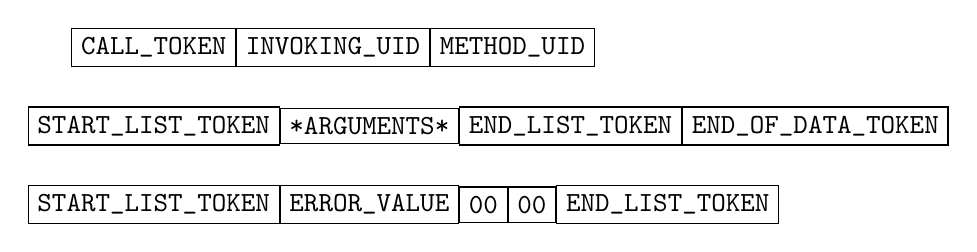
\begin{tikzpicture}
% \draw (0,0) rectangle (2,2) node[pos=.5] {\verb|CALL_TOKEN|};
\node[draw] (1) at (0, 0) {\verb|CALL_TOKEN|};
\node[draw] (2) [right = 0cm of 1] {\verb|INVOKING_UID|};
\node[draw] (3) [right = 0cm of 2] {\verb|METHOD_UID|};
\node[draw] (4) at (0, -1) {\verb|START_LIST_TOKEN|};
\node[draw] (5) [right = 0cm of 4] {\verb|*ARGUMENTS*|};
\node[draw] (6) [right = 0cm of 5] {\verb|END_LIST_TOKEN|};
\node[draw] (7) [right = 0cm of 6] {\verb|END_OF_DATA_TOKEN|};
\node[draw] (8) at (0, -2) {\verb|START_LIST_TOKEN |};
\node[draw] (9) [right = 0cm of 8] {\verb|ERROR_VALUE|};
\node[draw] (10) [right = 0cm of 9] {\verb|00|};
\node[draw] (11) [right = 0cm of 10] {\verb|00|};
\node[draw] (12) [right = 0cm of 11] {\verb|END_LIST_TOKEN|};
\end{tikzpicture}    
\caption{Caption}
    \label{fig:my_label}
\end{figure}

Both the invocation of the method and the respond use the same general structure. Response method uses parameters to return data.
There are two types of arguments: mandatory arguments that all have to occur in the specified order, and optional arguments which can be left out and each of them is formatted as follows: \\ \verb# START_NAME_TOKEN | ARGUMENT_ID | ARGUMENT_VALUE | END_NAME_TOKEN #.

% object UID can be SP, table, row of table of a special object UID, SMUID --- session manager, used for session management



\subsection{Sessions}

Whereas ComID is used to differentiate the senders and, therefore, also the recipients of the methods, sessions are used for parallelization of communication of one such actor. Each session can have different authorized authorities and methods in process, but each session is still bound to one ComID. Since each ComID corresponds to one user, both the user and the TPer can send multiple methods calls or responses in one ComPacket.

TODO: not user or actor but host... e.g.  if it would be network storage, there can be some thingie that would split the communication 

Sessions use a system of readers-writer locks to enable several concurrently running read sessions without causing concurrency issues.

There are two types of sessions: regular session and control session (not going to care about control much, just between the TPer session manager and host session manager)...
Each ComID has one associated control session with a lifespan the same as the ComID. On the other hand, there can be multiple regular sessions.

Since the control session is used to establish a regular session with an SP, it is not connected to any SP. The control session is used for managing the regular sessions and, as such, provides methods such as:
\begin{itemize}
\item The \verb|properties| method enables to find a compromise between the communication capabilities of the host and the TPer or simply find the communication capabilities of the TPer. Using this method, the properties defined earlier in section~\ref{TODO}, such as maximum packet size, are established.
\item The StartSession and SyncSession methods provide a way to start an unencrypted session.
% \item The StartTrustedSession and SyncTrustedSession methods provide a way to start an encrypted session. They are used if needed after a StartSession/SyncSession invocation to finish protocols requiring two passes, such as ...
\item The StartTrustedSession and SyncTrustedSession methods provide a way to complete challenge-response authentication or to setup secure messaging/key exchange.
\item The CloseSession method used to close the session.
\end{itemize}

Each is identified by it's session number. The session number consists of the TPer session number selected by the TPer and the host session number selected by the host.




\subsubsection{Secure messaging}

Depending on the authorities used, it is also possible to start a secure messaging session, which provides message authenticity and/or confidentiality.
Authority's operation type decides the what trusted messaging is to be used. These are further described in the section~\ref{TODO}.
With other cases there is no secure messaging.
% *trustedsession - used with PuK, SymK, and HMAC authorities, secure messaging

% During session initialization, using the method StartSession, there are parameters for four parameters for authentication. Host/SPSigningAuthority for explicit authentication and Host/SPExchangeAuthority for implicit authentication. 

% not about trusted session anymore...: it is also possible to explicitly authenticate more than one authority, using the Authenticate method.

% TODO: talk about ComID lifecycle

\subsection{Transactions}

In order to facilitate safe execution of sequences of methods, the standard specifies transactions. Similarly to transactions in database systems, this feature enables one to revert effects of sequence of methods. This is done automatically in case the transaction is not finished, or if the transaction is manually aborted. However, not all the effects of methods are rolled back, such as logs. Nested transactions are supported, in which case the transaction is committed when the outermost transaction is finished.

\subsection{Memory structures}

In order to maintain the state of the device, tables are exclusively used. Tables are defined by their columns and each row is called an object.
Each SP contains a meta table called Table table which contains information about all the other tables in the SP.

Each template also defines its tables such as the key tables containing keys for different LRs.

% move probably under templates,,, or even better SP?

\section{Access Control}

In order to provide access to methods only to authorized actors, the standard also defines access control. The access control provides a way to allow access to methods of the SP only after the knowledge of a secret has been proved. Information required to verify knowledge of the secret is called a credential and is stored in one of the corresponding SP's credentials tables. Each SP may contain several credential tables, one for each type of credentials, such as a password,  an RSA key pair, or an AES key.

In order to support authentication of more than one user or require multiple users at once, access control rules are defined using Access Control Lists (ACL) containing Access Control Elements (ACE). Each entry in an ACL has an owner \dots. ACEs are Boolean expressions with inputs being authentication of authorities.

Each combination of method and object has defined ACL, which needs to be satisfied in order for the method to be invoked on the object. An ACL is satisfied once one of the ACEs contained within it is satisfied, where authenticated authority variables evaluate as true.


% Access control -- access control list consists of access control elements (boolean combination of authorities),,,
% each SP has AdminExch authority,,, 
% ACEs seem to be able to have different "owners",,,

% Other than an explicit authentication, an implicit authentication is also possible. In this authentication, the knowledge of secret is shown by successfully using encrypted communication channel. FACT CHECK

Other than explicit authentication, implicit authentication is also possible. Implicit authentication may be used with, e.g. the Exchange operation type where the session key by the SP is encrypted using a pre-shared key and returned to the host.


Authority may be authenticated either during session startup using parameters of the SessionStart method, or, if there is more than one authority, the additional authorities may be authenticated using Authenticate method. 
The Authenticate method authenticates only using explicit methods. 
In case Authenticate method is used to authenticate using a password, one invocation of the method with a password as the parameter is enough. In the case of challenge and response operation type (Sign, SymK, HMAC), the first invocation only specifies the authority to be authenticated and receives challenge in response, and the second invocation provides the response.


Each authority is an object in the authority table of the corresponding SP.
Each authority has a type which is either individual or class. Class authorities correspond to a set of authorities so that they can be easily assigned and changed in bulk.

Other than the Admin and User authorities, there is also a special SID authority. This authority represents the owner of the TPer, and, as such, provides access of admins extended by the capabilities related to TPer management, such as the ability to activate an SP or enabling Admin authorities. Compared to the other authorities, SID authority is shared between all SPs.
There is also the Anybody authority that provides access to public information on the TPer. No authentication is needed for this authority.

Other than PIN authentication, the Core standard also defines other approaches to authentication.

\subsection{Authorities}

Authorities are constructs used to represent an actor. Authorities are saved in the Authority table of every SP, provided by the Base template, and so are separate for each of the SP. Each authority is associated with one credential. This credential is an object from a table, depending on the type of the credential.

The Base template defines several optional authorities such as the Admin authorities, representing the owner of the SP, the Makers authorities, representing the manufacturer of the TPer, the Security Identifier authority (SID), representing the owner of the TPer, and TPer authorities, representing the TPer itself.
The Base template also defines a special authority Anybody without any credentials. This authority can be used in reading public info of the SPs or to take ownership of the TPer.

% Other templates also define other authorities. Both  such as the User authorities from Locking template, ...

Each authority has assigned one operation type. This operation type determines how can this authority be used to authenticate.
\begin{itemize}
    \item None --- 
    \item Password --- also called PIN, authenticated using a password as a parameter.
    \item Sign --- authenticated using challenge and response with asymmetric crypto.
    \item Exchange --- credentials of this authority are used to encrypt session key. Can be used only in StartSession.
    \item SymK --- authenticated using challenge and response with symmetric crypto.
    \item HMAC --- challenge and response with HMAC. E.g. during session startup the HMAC is sent in a parameter and contains the HMAC of the method excluding the HMAC parameter.
    \item TPerSign --- used to authenticate the TPer.
    \item TPerExchange --- 
\end{itemize}


\section{Templates}

Since SPs may share some of their functionality such as authentication, modification of tables, or retrieval of data from tables, there exists templates to define this shared functionality. Each of the SP then implements a subset of functionality of one or more templates. Since templates 

\subsection{Base template}

The Base template defines the shared subset required by every SP, and is therefore mandatory. The most important functionality that is defined by this template is access control and metadata.

\subsection{Admin template}

The Admin template is a template specific for the unique Admin SP. It provides access to methods managing the TPer.

\subsection{Crypto template}

Template providing methods providing cryptographic methods.

\subsection{Locking template}

Template specific for the unique Locking SP. Provides access to methods managing the lock state of the device, locking ranges...

\subsection{Clock template}

Template providing methods for indicating current time, measuring lag, and access to monotonic counter. 

\subsection{Log template}

Template providing methods for logging activity. The logging can be either carried out manually by an user (or an user application) or automatically by the TPer (as a result of invocations of methods of SPs containing this template, including invocations during read-only sessions). 
Only one system log table may exist on each SP, but multiple user log tables may be present on one SP.
The logs are saved on non-volatile storage, depending on the security setting of the table, they may be either buffered or be saved after each entry.

% TODO: how much are the logs preserved... will they get deleted with an SP?

\section{Admin SP}

% There are two so called Manufactured SPs, SPs which are 

The first of the Manufactured SPs is the Admin SP.
This SP holds information about the TPer and all the present SPs, it allows creation, deletion and general modification of the SPs.
It is ses base and admin template

unique

This SP is initialized as "manufactured", so that it can function as a starting point of TPer management.

\subsection{Methods}

Even though the templates from which the Admin SP consists define many more methods, the Opal standard mandates only the following ones:
\begin{itemize}
\item ``Next'' --- returns UIDs of objects in the table. Allows to specify the returned amount and the first UID.
\item ``GetACL'' --- returns the ACL of the method and object or method and table combination.
\item ``Get'' --- returns the value of the object or the contents of the byte table.
\item ``Set'' --- sets the value of the object or the contents of the byte table.
\item ``Authenticate'' --- performs an additional explicit authentication.
\item ``Revert'' --- reverts the SP referred to by the invoking ID to its initial state.
\item ``Activate'' --- activates the SP referred to by the invoking ID.
\item ``Random'' --- returns specified amount of random bytes.
\end{itemize}

\section{Locking SP}

Locking SP procures the disk encryption and the locking and unlocking associated with it. This means that it provides access to manipulation of locking ranges, key generation and ...

also unique

uses base and locking template

\subsection{Methods}
Some of the methods Opal mandates for Locking SP are shared (``Next'', ``GetACL'', ``Get'', ``Set'', ``Authenticate'', ``Random''), but there are also two new ones:
\begin{itemize}
\item ``GenKey'' --- regenerates a key or a credential. But, in the case of Opal, this method is mandated to be able to be used at least on the \verb|K_AES_*| DEK keys.
\item ``RevertSP'' --- reverts the Locking SP. Compared to ``Revert'' this method can revert only the SP to which the session is connected, allowing reverting without having access to Admin SP's Admin authority.
\end{itemize}

\subsection{Locking range}

The locking range feature gives the user a way to specify an LBA range on the disk that can be locked independently on the rest of the disk. Each locking range also has its own ACE to control who can lock and unlock the range. Because each LR is also encrypted using its own DEK, it is possible to regenerate new DEK for a single LR, discarding data of only one LR.


There also always exists a special range called the global locking range that covers any area on the disk that is not already covered by a regular locking range.

In order to control the access to the data on a disk covered by a specific locking range, the Locking table contains columns ReadLockEnabled, WriteLockEnabled, ReadLocked, and WriteLocked. The data inside the LR cannot be read when ReadLockEnabled and ReadLocked are both set to true. Otherwise, the LR range is locked, and the data cannot be read. Similarly, for writing and WriteLockEnabled and WriteLocked. The separation of the locking right into the LockEnabled and Locked column gives the ability to have separate ACE for the LockEnabled column, meaning that, for example, an admin can decide that the user can only lock reading for a specific LR but not writing. 

Each locking range also has a defined column LockOnReset containing a list of types of resets on which the LR gets locked. Although there are defined types such as HotPlug (which is not really defined anywhere, but we suspect that it corresponds to the ATA Hot Plug reset)... Opal requires the support of only the Power Cycle, Programmatic\footnote{Activated by TPER\_RESET, command on TPer layer.} and optionally Hardware Reset reset.

\subsection{Single User Mode}

In many cases, it might be desirable to prevent admins from accessing user data, even though the admins generally have more competence. 
The Single User Mode Feature Set~\cite{tcg-sum} defines a way to achieve this.
After activating Single User Mode, only a single User authority is capable of changing their authority object (this includes changing their PIN), changing the proprieties of LRs assigned to them (which includes the lock state of the LR) and generating new keys for those LRs.
The only actions available to the Admin authorities related to that LR are destructive actions.

% feature set that ``locks'' the admin out --- admin can do only destructive actions upon the locking range, and only the user can actually unlock it

\subsection{MBR shadowing}

This feature enables the disk to provide a fake master boot record (MBR). Instead of the MBR saved on the disk, the disk instead provides the shadow MBR saved in a table on bootup. The shadow MBR may contain software to enable the host to authenticate itself to the disk and unlock it. After the host is authenticated, the shadow MBR may be deactivated, and the regular disk data will be available again.

This feature is controlled using tables \verb|MBR|, a byte table containing the data to be presented while the shadowing is active, and \verb|ControlMBR|, an object table used to control the shadowing. Table \verb|ControlMBR| one row with columns \verb|Enable|, \verb|Done|, and \verb|MBRDoneOnReset|.
When \verb|Enable| is true and \verb|Done| is false, the shadowing is active, and the data from \verb|MBR| table can be read from the disk. The column \verb|MBRDoneOnReset| specifies a list of types of resets during which the \verb|Done| is set to false.

% TODO: specify reset types?

% The minimal maximum size of the shadow MBR seems to be 0x08000000 bytes ($\sim$134 MB).

% Move to locking SP.



\section{Opal SSC}

Even though the Core specification introduces many powerful and interesting features, this might increase the cost of design and manufacturing of a fully compliant device. To solve this problem, the Opal SSC determines only a small set of mandatory features, leaving most of the features optional. Together with the set of mandatory features it also states range limits of certain properties.

For access control, Opal is mandating only password authentication, this means that any other authentication such as implicit authentication of the host or any authentication of the TPer (and therefore also secure messaging) may not be available. For communication Opal requires only support of synchronous communication. For table management, Opal does not require support of creation or deletion of tables. Issuance of SPs is also not required, and Opal instead uses SPs preconfigured by the manufacturer.
Out of the previously mentioned SPs, Opal requires only that the Admin SP and the Locking SP are supported. Since SP issuance is not one of the mandatory features, the Locking SP may also be preconfigured by the manufacturer and be initially in the ``manufactured-inactive'' state. 

Due to the range limits specified in the Opal SSC, the following features also might not be available.
\begin{itemize}
\item Opal specifies that the device must be able to handle: at least one method per SubPacket, at least one SubPacket per Packet, and at least one Packet per ComPacket. This means that any ...
\item At least one active transaction per session, at least one active session per all the ComIDs and at least one ComID.
\end{itemize}
This means that an Opal-compliant device implementing only the required minimum will also not be able to provide any

But Opal does not only reduce the feature set from the Core standard, but also expands it with some extra feature sets. Even though the Core specification does not require the following feature sets, the Opal SSC requires them additionally.
% 2.10 Mandatory Feature Sets
% An Opal SSC compliant SD SHALL support the following TCG Storage Feature Sets:
% 1) Additional DataStore Tables, Opal SSC Feature Set (refer to [6]);
% 2) PSID, Opal SSC Feature Set (refer to [6]).
% 3) Block SID Authentication Feature Set (refer to [8])
\begin{itemize}
\item Physical Presence SID (PSID) is a special authority that is authorized to call only the Revert method. The PIN of this authority may not be found out using the interface of the disk, every one of our disk supplied this information on a label on the disk. This authority provides a way to reset the TPer into factory state even in case the SID PIN is lost.
\item DataStore tables are byte tables accessible for any use. Using the Activate method, the number of the DataStore tables with their sizes can be specified.
\item Block SID Authentication feature disables SID authority until device restart. Can be used by BIOS to protect somehow... this functionality seems kind of a reach...
\end{itemize}

From our experience with Opal disks, most of them did not implement more than the required minimum (TODO: fact recheck later on). Some of the tested disks, even though they were described by the vendor and/or manufacturer as Opal-compliant, did not implement every required feature set. Out of the 6 tested disks, only 2 implemented the required Block SID Authentication feature set. However, even those 2 implementing the feature set did not support the actual feature.

% TODO: maybe there is a difference between supporting the feature set and supporting the feature?

% 4.1.1 Block SID Authentication Feature (Feature Code = 0402)
% This feature descriptor SHALL be returned when the SD supports the Block SID Authentication Feature Set. The
% contents of the feature descriptor are defined in Table 2.


\section{Host-side implementation}

Other than using generic SED software introduced in chapter~\ref{TODO}, there are more low-level approaches to controlling Opal hardware available, which offer more control over the device. In this section, we will introduce two such approaches available in Linux systems.

\subsection{Linux ioctl}

Since version 4.11 the Linux kernel offers set of ioctl requests to facilitate control over an Opal disk~\cite{linux-opal-introduction-mail}. Although these ioctl requests offer a simple access to control of the disk, not every feature mandated by Opal is implemented. Some of the limitations are the following: 
\begin{itemize}
\item Access to only single admin authority and up to 9 user authorities.
\item No way to change SID PIN. This means that the authority representing the owner of the device, that often has control over the entire disk, is stuck with the PIN that was chosen during the taking of the ownership.  
\item no "write only" lock
\item no configuration of lockout, and no way to reset lockout --- doesn't matter since opal has read-only lockout values -> not implemented
\item The last mentioned is the missing  ability to read or write to object table rows or iterating tables. This prevents the possibility of replacing the missing features using a direct setting of values in a table.
\end{itemize}

The individual implemented ioctl requests for Opal functionality and their function as of Linux kernel 5.19 are:
\begin{itemize}
\item \verb|SAVE| --- adds a key for a locking range into a unlock list, so that it can be used after waking the disk up from suspend. To wake the disk up, exported symbol \verb|opal_unlock_from_suspend| can be used to unlock the disk with the saved data. Note that the data is saved only in the RAM, and so this cannot be used to wake the computer (??? What did i mean by this?... anyway this is entry point for some vulnerability analysis because it basically gives us back the cold boot attack!).
\item \verb|LOCK_UNLOCK| --- locks or unlocks reading or writing for the selected locking range.
\item \verb|TAKE_OWNERSHIP| --- changes the admin authority password from the default one to the selected one. TODO: write about initialisation of the TPer to the generic chapter, \verb|C_PIN_MSID| etc.
\item \verb|ACTIVATE_LSP| --- changes state from "Manufactured-Inactive" to "Manufactured" state. Also facilitates setup of single user mode. TODO: write about TPer states in the generic chapter. 
\item \verb|SET_PW| --- changes the password of the selected authority, using the admin password.
\item \verb|ACTIVATE_USR| --- enables specified user in the Opal tables.
\item \verb|REVERT_TPR| --- reverts the TPer to the manufactured state using admin password.
\item \verb|LR_SETUP| --- sets locking range position/locking enable
\item \verb|ADD_USR_TO_LR| --- sets the ACE for locking and unlocking to the designated user. Does not actually add a user, instead replaces any existing one by the new one. % adds a user to the LR ACE. ...\verb|l_state == OPAL_RW| means writing ace...  (TODO: they seem to set it to "\verb#(user_uid || user_uid)#"??? why? bug? -> MRE is \verb|opal_util_linux.c|, only used last assigned to LR can control it, does (not) work on all test disks
\item \verb|ENABLE_DISABLE_MBR| --- changes \verb|Enable| parameter of the \verb|MBRControl|. % TODO: write about MBR in a generic chapter.
\item \verb|ERASE_LR| --- calls the erase method, 00 00 06 00 00 08 03, can't find it in opal and in core it's "reserved for SSC", ... it's in single user mode standard --- not only destroys data, also removes pin and user authority (for SUM).
\item \verb|SECURE_ERASE_LR| --- regenerate the data encryption key of a range to destroy the previous one.
\item \verb|PSID_REVERT_TPR| --- resets the TPer to the manufactured state using PSID.
\item \verb|MBR_DONE| --- changes \verb|Done| parameter of the \verb|MBRControl|, only when both the Done and Enable parameters are enabled, MBR shadowing is active.
\item \verb|WRITE_SHADOW_MBR| --- writes data into the MBR table.
\item \verb|GENERIC_TABLE_RW| --- reads a byte table or writes into a byte table. Neither object tables nor iteration are supported.
\end{itemize}

Currently, there is no documentation to be found for the ioctl requests for Opal functionality. The information in the previous list was acquired from our code analysis.
Short program showcasing the usage of this interface can be seen in the appendix~\ref{TODO}.

\subsection{Direct communication}
\label{direct_communication_raw_ioctl}

Alternative to the Opal ioctl requests are disk controller ioctl requests. Depending on the disk protocol, a different way of passing the Opal commands is required, such as using \verb|SG_IO| ioctl and \verb|sg_io_hdr_t| structure for SCSI disks or \verb|NVME_IOCTL_ADMIN_CMD| ioctl and \verb|nvme_admin_cmd| structure for NVMe disks. Using these structures, the Opal commands described in chapter \ref{TODO} can be sent to the TPer. Compared to the Opal ioctl requests this has the advantage of not being limited only to a subset of features that the Opal ioctl requests implement, and instead being able to use every Opal feature the device offers. This is not limited only to \dots (e.g. improve performance by using optional features such as concurrency, etc, described earlier) \dots

Although this approach gives the user access to every feature of the Opal disk, it also requires them not only to implement the command hand-over for each type of disk separately, but also to create the methods and parse the method results, both described in chapter \ref{TODO}, on their own.

TODO disk interface popsat\cite{NVME}

The commands that are called through the disk controller ioctl requests are called IF-RECV/IF-SEND in TCG Storage standards~\cite{tcg-storage-core}. These commands corresponds to several other commands in different interface specification. Some of them are the Security Receive/Security Send commands in NVMe~\cite{nvme-express-base-specification}, the TRUSTED RECEIVE/TRUSTED SEND commands in ATA~\cite{acs-3}, or the SECURITY PROTOCOL IN/SECURITY PROTOCOL OUT commands in SCSI~\cite{spc-4}.


 

\newcommand{\REPLACEME}{\subsection*{Impact on Opal devices}}

\chapter{Security of hardware encryption}
\label{chapter:security}

Disk encryption is usually not meant to protect the content of the device while it is being actively used.
For example, the Opal standard aims to only \enquote{Protect the confidentiality of stored user data against unauthorized access once it leaves the owner's control (following a power cycle and subsequent deauthentication)}~\cite{tcg-opal2}.
Even if the device is successfully protected against such a threat model, it still leaves many possible attack vectors.
To extend the threat model into a more realistic scenario, we consider an attacker that has physical access to the disk installed in a ``locked'' computer. We consider a computer to be ``locked'' if it is either turned off completely or protected by a lock screen or similar way of preventing unauthorized access to the computer.\todo[color=green]{what about servers?, i think that's good enough improvement}

% It should be noted that some systems 

% In order to limit the scope of the analysis, we will focus primarily on the hardware...
% The threat model we consider in this analysis is primarily going to be the same ...

% specify threat model, ,....,,, offline, online,,, offline multiple times???s

% .. maybe change position of this chapter, since it's splitting tools and change to a tool

% In this chapter we will look at several possible attacks against self-encrypting drives.

% \section{Attacks on hardware encryption}

In this chapter, we will provide an overview of state-of-the-art attacks relevant to hardware disk encryption. For each attack, we will provide our theoretical analysis of the protection offered by Opal, if properly implemented in a disk, against such an attack. For a selection of the attacks, we will also provide our practical insight. The set of disks we have tested is made from SanDisk X300s, Kingston KC600, Samsung SSD 850 PRO, Samsung SSD 860 EVO and Samsung SSD 980 disks.

% TODO: clean up with citations from the vulnerabilities papers\cite{bypassing_in_enterprise, got_hw_crypto, self_decrypting_risks, self_encrypting_deception, systematic_assessment_of_the_security}.

% something about the fact that we are providing a overview of state-of-the-art attack on hardware encryption.


\section{Evil maid attack}

An evil maid attack~\cite{self_decrypting_risks,systematic_assessment_of_the_security} consists of a situation where the device is left unattended for some time, during which the attacker has full physical access. Such attacks often have two phases. In the first phase, the disk is modified, e.g. by installing custom firmware or inserting a probe to eavesdrop on the communication. Then, the victim uses the disk, providing the password to unlock it. In the second phase, the attacker returns to collect the obtained information and undoes their changes. In some cases, the attacker might not require physical access to the device and instead use a network to receive information and have, e.g. the modified firmware reverse itself or simply leave traces if the discovery of the attack is not a problem.

\REPLACEME

For the two-phase type of the attack, the Opal disk itself has protection against unauthorised changes. The shadow MBR requires authentication to be changed, and although newer versions of Opal do not mandate an interface for firmware update anymore, it is standard practice to require a newer signed firmware to update.
But eavesdropping on the communication between the host and the drive is still possible, as Opal does not mandate secure messaging, and therefore any encrypted communication, it is still a real possibility to insert a probe in between the disk and the computer.

% Hmmm, maybe something like: Opal does not specify anything about firmware update, and shadow MBR update requires authentication. Still, one could still listen to the cables, I suppose because Opal does not mandate secure messaging and so the communication can be simply sniffed out on the ATA/NVMe/whatever cables?


In general, there is not much protection against evil maid that does not care about detection, as they need to only fake that the system is real until the password is acquired. They can replace the victim's machine with one that is similar enough until that time. This means that the disk itself can also be replaced, most likely circumventing any protection against such an attack on the disk.
Although physical security is the obvious solution, another approach is to let the disk verify itself first. Once again, the Core standard offers a way for the disk to authenticate itself to the host, but the Opal standard does not mandate that it will be supported.


An encrypted communication would be able to prevent the password from being sniffed by a probe between the disk and the host. For this purpose, the Core standard defines the secure messaging feature, which provides confidentiality of the communication.
Authentication of the disk to the host would be able to prevent the replacement of the disk. 
The core standard introduces this feature through different types of authority operations, such as challenge and response.
However, the Opal standard does not mandate secure messaging and the only authority operation it does mandate is a password, and so it is unlikely that any Opal device would implement them.


% An encrypted communication would allow preventing the password from being sniffed by a probe, and authentication of the disk to the host would prevent 
% These features are defined in the Core standard under secure messaging and as a method of authentication, respectively. 


% opal does not mandate secure messaging, which would allow encrypted communication, which would also require cold boot attack to acquire the encryption key, to get access to current session. But secure messaging is relevant only to the management of the disk, not to the direct reading writing, so as long as the LR would be unlocked this would not help........\todo{.........}



\todo[color=green]{anti-evil maid does not fit very well, removed it}
% Other than physical security, there exists a solution for this type of evil maid in the form of anti evil maid~\cite{https://blog.invisiblethings.org/2011/09/07/anti-evil-maid.html}, which uses a trusted boot in order to authenticate the machine to the user before the user authenticates themselves to the machine.



\section{Attack on key generation}
\label{attack_rng}

An attack on key generation is such an attack which abuses the RNG generating data with low entropy or even entirely predictable. Due to the decreased entropy, it may be possible to potentially predict the value of the DEK~\cite{self_encrypting_deception}.
% Such vulnerabilities are not unprecedented. \cite{got_hw_crypto}
Since Opal specification does not actually specify any implementation for the RNG, we cannot perform any fruitful analysis of the standard itself. However, we can still try to perform practical analysis.


\REPLACEME

The Opal specification offers a few ways how to generate random data. The most useful would be GenKey, as it is used for generating DEKs, but since the destination cells, where the result is recorded, are protected from reading, we cannot easily read them to get the generated values.
Another method of generating random data is the method Random. This method allows us to get at least 32 bytes~\cite{tcg-opal2} every invocation. Even though the RNG used by this method might be different to the one used by the GenKey method to generate DEKs and has low performance (our slowest tested disk was able to generate about 500 bytes per second), the Random method provides easy access to the generated data.
To test the randomness of the RNG of the disks, we have decided to use the Random method and \emph{dieharder}\footnote{\url{https://webhome.phy.duke.edu/~rgb/General/dieharder.php}} statistical randomness tests battery.
From the disks we have inspected, we have found the following about their RNG:
\begin{itemize}
    \item \emph{SanDisk X300s} always generates the same bytes for the first Random invocation of a session. The value of the first bytes seems to change only after the new activation of Locking SP. Following invocations of the Random method in a single session return different bytes. This weakness does seem to also affect the key generation. We tested this by zeroing out several blocks of the drive and re-generating the DEK. Each time we re-generated the key, the drive content was different. However, we have decided to also test the randomness of the content. If we zeroed out the content before the key re-generation, the content did not pass the test of randomness. If we, however, wrote random data before the key re-generation, the content did pass the randomness test. This property was different from every other disk and may suggest that the key generation is truly not entirely random. When looking closer at the contents of the disk generated this way, it is possible to see several patterns described more closely in Appendix~\ref{appendix:rng_pattern}.
    \item \emph{Kingston KC600} generates data that passes most of the dieharder tests, even though the Random method requires extra consideration while it is being invoked. The Random method of this does not actually accept parameters as atoms but as unsigned integers. However, this does not cause a difference in behaviour as long as the value of the atom is small enough. 
    % \item \emph{Samsung SSD 850 PRO, Samsung SSD 860 EVO and Samsung SSD 980} generate random data that passes most of the dieharder tests, for which enough data was generated.
    \item \emph{Samsung SSD 850 PRO, Samsung SSD 860 EVO and Samsung SSD 980} generate data that passes most of the dieharder tests. % passed for the generated data\todo{recheck for all actually....}.

\end{itemize}

Regarding the generated data not passing every test, as the generation of random bytes takes a considerable amount of time, we have generated only a limited number of bytes for the test. The limited size of the data set is most likely the cause of some tests not passing, as these tests have reused the input data.


    % \item \emph{Samsung SSD 850 PRO, Samsung SSD 860 EVO and Samsung SSD 980} generate random data that passes most of the dieharder tests. % passed for the generated data\todo{recheck for all actually....}.


% Using this method, we have decided to generate random bytes to inspect later.\todo{what about testing by reading the disk directly??? }
% In order to test these generated numbers we have decided to use the \emph{dieharder}\footnote{\url{https://webhome.phy.duke.edu/~rgb/General/dieharder.php}} random number tester.

\todo{something how not everytinh buit a large majority of diehard tests passed but that's expected and most likely because of small amount of data}


\todo{maybe move the appendix here? to make the own text bigger :))))}%\todo{check out if this is not just cbc thing, since this one is the only non-xts}
    % \item Kingston KC600 --- for the minimum 32 bytes, the TPer closes the session on Random invocation. The same response was for most of the other tested values. However, if exactly $256^n-1$ bytes are requested, $128+n$ bytes are returned... lol, I see where the problem is now. The TPer doesn't parse it as a token but as a regular ``C'' unsigned integer. So, it was reading the header instead, and the \verb|0xff| bytes were required for ``NOPs'' since they are tokens for empty atoms. With a slight modification, we can get up to 255 bytes from this disk at once.

 %  generate data although this drive does not parse the Random method correctly, not being able to parse the header of the number atom, 
% all dieharder tests passed.
%  for the minimum 32 bytes, the TPer closes the session on Random invocation. The same response was for most of the other tested values. However, if exactly $256^n-1$ bytes are requested, $128+n$ bytes are returned... lol, I see where the problem is now. The TPer doesn't parse it as a token but as a regular ``C'' unsigned integer. So, it was reading the header instead, and the \verb|0xff| bytes were required for ``NOPs'' since they are tokens for empty atoms. With a slight modification, we can get up to 255 bytes from this disk at once.

% Note that for the testing of SanDisk X300s' RNG, we did not include the first batch of random bytes that were always the same, as they would spoil the perceived randomness of the rest of the numbers.

% SanDisk X300s --- However, using GenKey on a locking range does change the data into random bytes, so it does not seem this affects key generation.

\section{Cold boot attack}
\label{cold_boot_attack}

In this attack, a property of volatile memories is used. Even though volatile memories lose the data stored in them after powering off, they do not lose the data instantly. This introduces the cold boot attack, which takes advantage of this fact. One of the ways this attack can be implemented is to take a RAM stick from the victim's locked computer and install it into the attacker's computer, where it can be read. Another possible approach is the reboot the victim's computer into the attacker's system~\cite{self_decrypting_risks}.

\REPLACEME

Even though this attack works quite well against software-based disk encryption and software encryption in general, against purely SED, it does not work that effectively. This is because, compared to software encryption, there is no need to store the encryption key in the computer's memory. The key is instead stored in the memory of the disk controller, where it can be physically protected against removal.
% .. (and also, it's not a generic RAM stick). 
However, this advantage holds only for the case where the key or the disk password is truly not kept also in the computer's memory, which may not always be the case with SEDs. In the Linux Opal ioctl commands introduced in an earlier Section~\ref{section:opal_opal_ioctl}, there is introduced a functionality to save the password for locking range in the memory. This functionality is introduced in order to allow the computer to wake from suspension automatically since the disk might need to be unlocked in such a case. But since the key is stored in the computer's memory, it is possible to acquire it using the cold boot attack.

\section{Hot plug attack}

Hot plug attacks are attacks similar to cold boot attacks. However, compared to the cold boot attacks, where the RAM is inserted into the attacker's system before the data in it is naturally destroyed, hot plug attacks instead move the disk into the attacker's system. This attack abuses the fact that SATA disks often have a data cable and a separate power cable. Because of this, it is possible to switch the data cable into a different host device without powering the disk off and therefore locking it~\cite{self_decrypting_risks}. 

However, this approach is certainly not limited only to SATA disks with separate data and power cables, as it is possible to translate the attack to many different physical disk interfaces. An attack called hot unplug attack~\cite{bypassing_in_enterprise} generalised this attack. 
Before unplugging the original cable with the power pins, substitute power pins can be connected together with the original ones, keeping the disk device powered while the original cable gets unplugged. 
% Since in this case the power is never interrupted, it also means that the disk does not 


\REPLACEME

The Core standard introduces HotPlug as one of the reset types. This event might seem like a possible solution to such attacks. However,  its meaning is not defined in the standards. TCG Storage Interface Interactions Specification~\cite{tcg-siis}, the standard defining, among other things, the mapping of reset types to disk interface events, does not mention the HotPlug reset type. None of the disks we have tested supported this reset type, so we are left to only speculate about its possible efficacy.

% not mandated is also HotPlug reset type, which could be most likely easily bypassed , but we couldn't test it ....as none of the disks we tested implemented this reset type.
% Another approach to prevent such types of attacks might the with usage of watchdog maybe, but that is something not implemented 



% Instead of reconnecting the original data cable, a new cable is ``connected'' together with the original one, and the original one is afterwards removed. The 

% \todo{
% In the Core standard~\cite{tcg-storage-core}, there exists a reset type called HotPlug. 
% Although this reset type is not described closer than the name in the standards, it most likely refers to the ATA/NVMe? hot plug TODO\cite{TODO}... 
% Using this reset type, it could possible to set an LR to lock when a hot plug is detected. However, as this reset type is not mandatory (nor optional) for Opal devices, and none of our Opal devices implemented it, we were not able to examine this solution further.
% However, even if the device would implement the HotPlug reset type, using it to prevent the hot plug attack would not be advisable as the hot-plugging process could be disabled in the attacker's system.

% There exist tools for that 
% }
% TODO: actually check this...


\section{DMA attack}

These attacks use the DMA interface, such as Thunderbolt or PCIe, to read the DEK from the host's memory or to circumvent the lock screen~\cite{self_decrypting_risks}. 

\REPLACEME

As long as the DEK is not in the host's memory, the first approach can be prevented. Although, as we mentioned in Section~\ref{cold_boot_attack}, this might not always be the case, even with SEDs.
The second approach can be hard to prevent on the SED side, 
However, modern systems already have implemented protections against such attacks, so the risk of such an attack might already be minimised.


\section{Vulnerable interface}

An attack on the interface is such an attack where problems in the interface are taken advantage of.
This might include attacks such as using vendor commands to read the disk directly, even if the disk is locked. In the past~\cite{self_encrypting_deception}, some hardware-encrypted disks were vulnerable to such attacks, allowing the usage of undocumented vendor commands to change the firmware of the device to a custom-made one. %requiring only the usage of undocumented vendor commands to read 
% either the data of the encryption module (in some cases containing the unencrypted DEK) or even the content of the disk itself.

\REPLACEME

As can be seen from the previous Subsection~\ref{attack_rng}, the implementation of the interface is not perfect for some of our tested disks. Even though issues like the disk expecting a different type of format are not directly connected to security in our case, such problems might be a sign of other issues possibly related to security.
% Something like non-security issues might very likely be a sign of possible security issues, so don't take those problem that we found lightly! Maybe also something that more information can be found in the data chapter or something like that.

This might be especially a problem if such a malfunctioning interface gives its user a false sense of confidence. While testing our disks, we found several interface flaws with Kingston KC600. One such flaw is the fact that the disk accepts any value as a reset type. While specifying types of resets that should lock a specific interface, it is possible to specify any type, not only types that are not supported but also types which are not even defined in the standards. This means that after ``successfully'' setting LR to be reset after a hot plug event, it might never actually be locked once such an event happens.

\todo[color=green]{rethink the subsection name., i think now it is good enough.... maybe}


\todo[color=green]{removed the variatons since they are not that interesting.... *i* think}
% \section{Variations of the previous attacks}

% In the Bypassing Self-Encrypting Drives (SED) in Enterprise Environments paper~\cite{bypassing_in_enterprise} several variation of the previously mentioned attacks are introduced.\todo{probably juts remove, or mention a little bit}
% One of those attacks is the Forced Restart Attack, similar to the Cold Boot attack, but using system crash. 

% \todo[color=green]{Another one is the Key Capture Attack, similar to the Evil Maid Attack~\cite{bypassing_in_enterprise}.
% }
% TODO: describe reset types in locking range section...


\chapter{Existing tools}
\label{chapter_tools}

In order to give users the ability to manage their SED disks without the need to create their own programs to access existing interfaces, there exist several tools implementing the protocols introduced in Chapter~\ref{chapter_hardware_disk_encryption} and Chapter~\ref{chapter_opal}. 

Note that some of the the tools use ATA TRUSTED commands for managing ATA Opal devices. When using these commands, it is necessary to first set the \verb|allow_tpm|\footnote{The usage of TPM in the name appears to be purely a historical blunder as it does not seem to be ever used for TPM, a cryptoprocessor standard defined by TCG, the same group defining TCG Storage standards.} flag of the kernel libATA library to allow Trusted Computing commands~\cite{acs-3}. This can be done either by specifying it as a kernel flag \verb|libata.allow_tpm=1|\footnote{\url{https://wiki.archlinux.org/title/Self-encrypting_drives}}.\todo[color=green]{where to find the instructions?, \url{https://wiki.archlinux.org/title/Self-encrypting_drives}}

% Some disks might provide their own software for their own proprietary hardware encryption. These are usually found separately on website or something, but some are provided as by the disk on an unecrypted partition.
In this chapter, we will look at several existing popular open-source tools that allow one to manage the encryption of disks.

% \section{Cryptsetup}

% \emph{Cryptsetup}\footnote{\url{https://gitlab.com/cryptsetup/cryptsetup}} is a tool for disk encryption setup. Although this tool supports several formats and volumes, such as ..., all of them are software, and there is no hardware encryption support as of now.\todo{probably remove this since it does not support any hardware encryption,,, yet}

\section{hdparm}
 
The \emph{hdparm}\footnote{\url{https://sourceforge.net/projects/hdparm}} tool provides a command line interface to control the parameters of ATA disks. Among others, this tool gives access to control ATA Security Feature Set.
The examples of SED-relevant commands for the functionality described in Subsection~\ref{subsection:enc_ata} are:
\begin{itemize}
\item Enable the ATA Security Feature Set:\\ \verb|hdparm --security-set-pass pwd /dev/sda|
\item Disable ATA Security Feature Set:\\ \verb|hdparm --security-disable pwd /dev/sda|
\item Unlock the disk:\\ \verb|hdparm --security-unlock pwd /dev/sda|
\item Erase the disk:\\ \verb|hdparm --security-erase pwd /dev/sda|
\end{itemize}
Implicitly the user password is referred to in the commands, but \verb|--user-master| can be specified to select master or user password explicitly. While enabling the ATA Security Feature Set, it is also possible to use the \verb|--security-mode| option to choose between high and maximum security modes.
A command to lock the drive is missing because a drive with an enabled ATA Security Feature Set is locked when powered off.

% ATA Security Feature Set: seems to be juts for ata and ata password, can it also work with our disks?

\section{sedutil}

\emph{sedutil}\footnote{\url{https://github.com/Drive-Trust-Alliance/sedutil}} is a tool for the management of SED disks maintained by the Drive Trust Alliance.
It currently supports the Enterprise and Opal SSCs (and additionally the remaining Pyrite, Opalite and Ruby SSCs in a fork of the project\footnote{\url{https://github.com/ChubbyAnt/sedutil}}) and NVMe and SATA interfaces.

Even though it is currently the most prominent open-source project to control SED disks, being exclusively used in guides for using SED on Linux, the code repository is inactive.\todo[color=green]{exclusively as it is the only one mentioned, not that it is not mentioned elsewhere..., hmmm , sounds fine i guess}


This tool does not use the Linux Opal ioctl interface and instead uses the approach described in Section~\ref{section:direct_communication_raw_ioctl}. This allows the tool not only to be multi-platform but also to use the Opal features in their entirety instead of only the subset introduced in the Opal ioctl interface.
% ... although there currently certain limits for e.g. having only one admin ...

% Provides functionality to:
The tool offers the following commands, grouped by their functionality:
\begin{itemize}
    \item Discovery: \begin{itemize}
\item \verb|isValidSED| command lists SSCs supported by the selected disk, the name of the disk and its firmware version.
\item \verb|scan| command performs \verb|isValidSED| command on every disk in the system.
\item \verb|query| command performs Level 0 and Level 1 Discovery on the selected disk.
\item \verb|printDefaultPassword| command prints the MSID password of the selected disk.
    \end{itemize}
    
    \item TPer management: \begin{itemize}
\item \verb|initialSetup| command takes ownership of the disk, initializes the Locking SP and the global LR, and enables MBR.
\item \verb|setSIDPassword| command changes the password of the SID authority.
\item \verb|setAdmin1Pwd| command changes the password of the Locking SP's first admin authority. 
\item \verb|setPassword| command changes the password of any supported Locking SP's authority.
    \end{itemize}
    
    \item Locking range management: \begin{itemize}
\item \verb|listLockingRange| command prints information about a single LR, such as the start, length or lock status.
\item \verb|listLockingRanges| command prints information about all LRs, similar to the previous command \verb|listLockingRange|.
\item \verb|rekeyLockingRange| command re-generates the selected LR's key, destroying the data in the LR in the process.
\item \verb|setupLockingRange| command sets the start and length of the locking range.
\item \verb|setLockingRange| command sets ReadLocked and WriteLock of the LR depending on the chosen configuration (read-write, read-only, or locked).
\item \verb|enableLockingRange| command sets ReadLockEnabled and WriteLockEnabled of the LR. 
\item \verb|disableLockingRange| command unsets ReadLockEnabled and WriteLockEnabled of the LR. 
    \end{itemize}
    
    \item Shadow MBR management: \begin{itemize}
\item \verb|setMBREnable| command sets Enable column of the MBRControl table.
\item \verb|setMBRDone| command sets the Done column of the MBRControl table.
\item \verb|loadPBAimage| command writes the contents of a file into the MBR table to be used as the shadow MBR.
    \end{itemize}

\begin{samepage}
    \item Reverting the device: \begin{itemize}
\item \verb|revertTPer| command reverts the TPer using the SID authority.
\item \verb|yesIreallywanttoERASEALLmydatausingthePSID| or the undocumented \verb|PSIDrevert| command reverts the TPer to factory state using the PSID password.
\item \verb|revertNoErase| command reverts only the Locking SP, keeping the global range data.
    \end{itemize}
\end{samepage}
    
    \item Enterprise-specific functionality\todo[color=green]{actually find out what the bands are first, seem like just locking ranges, but hard to find source, .... yea}: \begin{itemize}
\item \verb|setBandsEnabled| command enables the usage of all locking ranges.
\item \verb|setBandEnabled| command enables the usage of selected locking range.
\item \verb|eraseLockingRange| command cryptographically erases the data in a specified locking range.
    \end{itemize}
\end{itemize}

% For Discovery there are commands 
% \verb|isValidSED| which lists supported SSCs by the selected disk,
% \verb|scan| which performs \verb|isValidSED| command on every disk in the system,
% and \verb|query| which performs Level 0 and Level 1 Discovery on the selected disk.
% Command \verb|printDefaultPassword| prints the MSID password.
% For management of the disk there are commands \verb|initialSetup| enabling to take ownership of the disk, 
% \verb|setSIDPassword| changing the password of SID authority,
% \verb|setAdmin1Pwd| changing password of Locking SP's first admin authority, 
% and \verb|setPassword| changing the password of any Locking SP's authority.

% For management of LRs there commands
% \verb|listLockingRanges| prints information about all LRs,
% \verb|listLockingRange| prints information about a single LR,
% \verb|rekeyLockingRange| regenerates the LR's key (destroying the data in the LR in the process)
% \verb|setupLockingRange| sets the start and length of locking range,
% \verb|setLockingRange| sets read locked and write locked of the LR, and
% \verb|disableLockingRange| and \verb|enableLockingRange| reading/writing locking enabled, 


% For controlling the shadow MBR there are commands \verb|setMBREnable| and \verb|setMBRDone| to set the Enable and Done columns respectively, and \verb|loadPBAimage| to write a file into the MBR table to be used as the shadow MBR.

% There are several commands for reverting the state of the device. Command
% \verb|revertTPer| reverts the TPer using the MSID password, 
% \verb|yesIreallywanttoERASEALLmydatausingthePSID| reverts the TPer using the PSID password, 
% and \verb|revertNoErase| reverts only the Locking SP, keeping the global range data.

% TCG Enterprise specific functionality, replaces LRs???? not really???, the use bands and bandmasters and erasemasters.
% \verb|setBandsEnabled|
% \verb|setBandEnabled|
% \verb|eraseLockingRange| 

\section{go-tcg-storage}

\emph{go-tcg-storage}\footnote{\url{https://github.com/open-source-firmware/go-tcg-storage}} is a Go library for managing TCG Storage disks, also providing CLI tools. Even though when compared to the previously introduced sedutil, it is not as popular, it is currently in active development. It supports not only Opal 2.0 and Enterprise SSCs but also Ruby, the successor of Enterprise. It also, compared to sedutil, supports, in addition, the SAS interface.
Although it implements a CLI, its capabilities compared to sedutil are very limited, as can be seen from the following paragraphs. The CLI consists of three utilities: \verb|sedlockctl|, \verb|tcgdiskstat|, and \verb|tcgsdiag|. 
For some of the tested disks, the utilities were not able to start a session due to time out and therefore function correctly.


The \verb|sedlockctl| utility allows one to control a SED disk. At the time of writing it offers the following commands: \begin{itemize}
 \item \verb|list| command lists all LRs.
 \item \verb|lock-all| command locks all LRs.
 \item \verb|unlock-all| command unlocks all LRs.
 \item \verb|mbrdone| command sets the MBRDone cell to the desired value.
 \item \verb|read-mbr| command prints the shadow MBR.
\end{itemize}

The \verb|tcgdiskstat| utility provides information about supported SSCs and firmware version for each disk, similar to the sedutil's \verb|scan| command. Unlike sedutil's \verb|scan|, it also prints whether encryption is supported, MBR is enabled, or SID authority is blocked.

The \verb|tcgsdiag| utility performs Level 0 and Level 1 Discovery, similar to sedutil's \verb|query| command. It also prints the MSID password, random numbers generated by the disk, and contents of the TPerInfo table. 


% \todo{that does everything, and is actually supported.}
\todo[color=green]{It has a few tools that let you do some things. It also supports more SSCs than others. Just found out about it, will need to look into it deeper and figure out why is it worse, so we won't look as bad.}
\todo[color=green]{CLI: Was able to generate random numbers, but only for some of the disks. and very limited control over it}

\section{TCGstorageAPI}

Seagate's \emph{TCGstorageAPI}\footnote{\url{https://github.com/Seagate/TCGstorageAPI}} is a library that provides a Python interface and a CLI tool. Similarly to sedutil, it supports Opal and Enterprise SSCs.
Compared to the previous tools, this one offers the most functionality, but this comes at the cost of also the largest dependencies. The tool has the most complete support for Enterprise SSC.
The library also includes a command to test an implementation of Opal drive, although it is not as complete as the test cases published by TCG.

% Something something something something something. something something something something. 

When used with a device implementing Opal 1 SSC, the CLI tool reported ``SED configuration is Unknown/Unsupported (Type Opal) - Exiting Script'', even though the device also implemented a supported Opal 2 SSC.
\todo[color=green]{CLI: doesn't work with sdc "SED configuration is Unknown/Unsupported (Type Opal) - Exiting Script", no random numbres} 

% \todo{Provides a Python library, written in c++, and a CLI...}

% \todo{Has a bunch of dependencies, most importantly boost, which is pretty big...}


\todo[color=green]{offers test suite!!!}

\section{sedcli}

\emph{sedcli}\footnote{\url{https://github.com/sedcli/sedcli}} is a tool for managing SED devices. Although the only supported disk interface is NVMe and the only supported SSC is Opal, it offers support for the Key Management Interoperability Protocol and key management servers.

\section{fscrypt}

Since inline encryption requires an active participation of the host during the encryption, a support in the kernel is required.
This means that in order to provide inline encryption it is not enough to have a user space tool.

\subsection{Kernel space library}

In the upstream Linux, there exists a support for inline encryption. However, it is currently used only by the kernel space library \emph{fscrypt}.
This library works on a filesystem level, which allows it to be more flexible compared to block device-level encryption, as it can limit the encryption to only some files. However, fscrypt does not encrypt all information of the files, and the metadata (excluding the filename) are left unencrypted.
Although by default fscrypt uses software encryption, it is possible to switch to inline encryption.

% The steps to activating inline encryption are described in more detail late in Chapter~\ref{chapter_tools}.
% There also exists a user space application with the same name\footnote{\url{https://github.com/google/fscrypt}}, that can be used to control encryption of file systems using kernel space fscrypt.


\subsection{User space tool}
% TODO: test CLI fscrypt...

\emph{fscrypt}\footnote{\url{https://github.com/google/fscrypt}} is also the name of a user space tool for the management of Linux filesystem encryption. Although it does not provide explicit support for inline encryption, thanks to the kernel space library fscrypt providing inline encryption in a transparent way, it can still be used to manage file system encryption with inline encryption.

% Even though the \emph{fscrypt} tool does not provide a way 
% Since the kernel space library fscrypt provides inline encryption in a transparent way, it is possible to use it 
% The user space library \emph{fscrypt} offers a way to configure an inline encryption for a given file descriptor. No CLI is provided and so the C library must be used instead.

As of now, block layer inline encryption is supported only by two file systems in Linux: ext4 and F2FS. 
In the following paragraphs, we will focus only on the ext4 filesystem.

First of all, inline encryption needs to be enabled in the kernel configuration. This means that the Linux kernel configuration option \verb|CONFIG_FS_ENCRYPTION_INLINE_CRYPT| needs to be enabled.
In order to start using inline encryption on a file system, it needs to be mounted with the option to specify the usage of inline encryption.
\begin{lstlisting}[language=bash]
mount -t ext4 /dev/foo /mnt/foo -o inlinecrypt
\end{lstlisting}
It is not enough to only specify the inline encryption flag. The encryption itself also must be enabled in the file system. On ext4 file systems, the encryption can be enabled after mounting like so:
\begin{lstlisting}[language=bash]
tune2fs -O encrypt /dev/foo
\end{lstlisting}
After this, fscrypt can be used as usual, and it will use inline encryption for this filesystem.
% Although it is possible to use the kernel space fscrypt library directly, there exist a user space utility with same name.

% In order to encrypt a folder using the kernel space fscrypt, the following must be done: an encryption key must be added and the encryption policy must be created. In C, this can be done the following way:
% \begin{lstlisting}[language=c]
% int fd = open(pathname, O_RDONLY | O_CLOEXEC);

% // add a key
% struct fscrypt_add_key_arg *key_request = calloc(1, sizeof(struct fscrypt_add_key_arg) + key_len);

% key_request->key_spec.type = FSCRYPT_KEY_SPEC_TYPE_IDENTIFIER;
% key_request->key_id = 0;
% key_request->raw_size = key_len;
% memcpy(key_request->raw, key, key_len);
% ioctl(fd, FS_IOC_ADD_ENCRYPTION_KEY, key_request);

% // set a policy
% struct fscrypt_policy_v2 policy_request = { 0 };

% policy_request.version = FSCRYPT_POLICY_V2;
% policy_request.contents_encryption_mode = FSCRYPT_MODE_AES_256_XTS;
% policy_request.filenames_encryption_mode = FSCRYPT_MODE_AES_256_CTS;
% policy_request.flags = FSCRYPT_POLICY_FLAGS_PAD_8 | FSCRYPT_POLICY_FLAGS_PAD_16 | FSCRYPT_POLICY_FLAGS_PAD_32;
% memcpy(policy_request.master_key_identifier, key_request->key_spec.u.identifier, FSCRYPT_KEY_IDENTIFIER_SIZE);
% ioctl(fd, FS_IOC_SET_ENCRYPTION_POLICY, &policy_request);
% \end{lstlisting}
% This code sets up an encryption policy for the file specified by the pathname. 



\todo[color=green]{probably rework into text about the tool for management instead?.......}
\todo[color=green]{requires the filesystem to actually use the library In the following paragraphs, that should be redone, I am assuming ext4......}

% \subsection{Usage}


% \subsection{Implementation}
% \todo{maybe remove completely?, doesn't seem to fit much...}

% During mounting the ``inlinecrypt''/\verb|SB_INLINECRYPT|  flag is written into the \verb|super_block| structure.

% It all starts in \verb|__ext4_new_inode|. This is the internal function used when creating new inodes, called by functions such as \verb|ext4_create| when creating a new file.

% The function (if it is not inode used for large extended attributes?) calls \verb|fscrypt_prepare_new_inode|.

% \verb|fscrypt_prepare_new_inode -> fscrypt_setup_encryption_info ->| \verb|setup_file_encryption_key ->  fscrypt_select_encryption_impl|

% In \verb|fscrypt_select_encryption_impl| there is actually the only place where the \verb|SB_INLINECRYPT| flag is used.
% ... Calls \verb|blk_crypto_config_supported| to check the device's crypto profile.
% Afterwards, \verb|fscrypt_select_encryption_impl| function sets the \verb|(fscrypt_info *)ci->ci_inlinecrypt|.

% \verb|setup_per_mode_enc_key| then sets the \verb|(fscrypt_info *)ci->ci_enc_key|.

% \paragraph{fscrypt - How does it work? - Usage}

% The bio function is stored in \\ \verb|(struct bio *)bio->(struct bio_crypt_ctx *)bi_crypt_context|

% Function \verb|fscrypt_set_bio_crypt_ctx| changes the file's bio to use inline encryption... simply calls the blk layer \verb|bio_crypt_set_ctx|.

% Calling \verb|submit_bio| like normally ... \verb|__submit_bio| calls \verb|__blk_crypto_bio_prep|...

% \blockquote{If the bio crypt context provided for the bio is supported by the underlying device's inline encryption hardware, do nothing.}

% \verb|__blk_crypto_rq_bio_prep| however sets the context of the request to the one of the bio... 
% After the bio prep  \verb|blk_mq_submit_bio| gets called (which calls \verb|blk_mq_bio_to_request|, and after that also \verb|blk_crypto_init_request->blk_crypto_get_keyslot| which updates the devices keyslot to contain the new key..., but does nothing if the device does not have keyslots)..... the info about the key to use then has to be acquired by the driver from \verb|request->|


% Most important are probably structures \verb|blk_crypto_ll_ops| and \verb|blk_crypto_profile|... just two operations, program key and evict key. 



% how to get crypto profile from outside..




% Where does the hardware come to play?

% \verb|ufshcd_exec_raw_upiu_cmd()->ufshcd_issue_devman_upiu_cmd()->ufshcd_prepare_req_desc_hdr()->ufshcd_prepare_req_desc_hdr_crypto()| sets the header with the correct keyslot.



\chapter{Opal toolset}

\todo[color=green]{implement proof-of-concept low-level tools to access available devices,}

In order to be able to study the self-encrypting drives, specifically the most popular Opal drives, at a closer level, we have implemented a toolset for controlling and inspecting Opal devices. 
We have focused on implementation that would not require any additional tooling or libraries and would allow as much control over the communication with the Opal device. This approach allows the project to be not only used on a system without introducing a plethora of additional packages but also for our code to be used in other projects without needlessly increasing the number of dependencies.
\todo{pridat --help do prilohy}

\section{Structure}

The code base is split into three levels. Each level implements a different part of the functionality that depends on the previous levels.

The lowest level is focused abstraction of the communication primitives. This includes primarily functions to build a method to be sent to the device and parse the received response, generic functions to start a session or set a value in a row of a table, and the implementation of IF-SEND and IF-RECV commands abstracting ATA and NVMe system calls.

% The middle level implements entire functions, like setup tper... 

The middle level joins the lower-level methods into complete functions. Each function represents one of the methods and provides a C interface to invoking the method. Internally the functions start a session with the device, build the method according to the function's arguments, send the method to the device, retrieve the response, and parse the response, to find whether to command was successful and to potentially return the data to the caller.

Finally, the top level combines the two previous levels to create a usable front end usable through a command line.

\section{Provided utilities}

Currently, there are implemented three front ends: \verb|rng| to produce random numbers generated by the selected Opal disk, the \verb|control| to manipulate the status of the selected Opal device, and the \verb|discovery| to inspect the selected Opal device.

\subsection{Random number generation}

\begin{figure}
    \centering
\begin{lstlisting}[language=Bash]
# ./rng /dev/sdb 24 2
e993f67588190fc5d6d0ef7c7febf1944c566e211ba10352
29b0897bb4ddec1d71d89c95fc945a031574936c3c687477
\end{lstlisting}
    \caption{Usage and output of the \texttt{rng} utility}
    \label{fig:rng_output}
\end{figure}

The \verb|rng| is the most straightforward front end of the introduced three. Its only goal is to produce random numbers generated by the disk quickly. However, all the disks we have tested implemented only the minimal Opal requirements, which guarantee a limit of only one active session, packets containing only one method, and the Random method providing only 32 bytes at once. Such properties do not leave much space for optimisation. The throughput this utility can achieve with the disks tested by us is between 500 bytes per second and 35000 bytes per second, depending on the disk. Although to obtain a sufficient amount of data, a considerable amount of time is required, this utility may be used to collect random numbers for testing the randomness of the disk's RNG.
The program repeatedly opens sessions, and during each session, it repeatedly sends the Random method. The total number of sessions and the number of bytes acquired during each session can be specified using the arguments as shown in Figure~\ref{fig:rng_output}.

\subsection{Device management}

\begin{figure}
    \centering
    \begin{lstlisting}[language=bash]
# reset device to the manufactured state
./control psid_revert /dev/sda \
    --verify-pin $PSID
# take ownership over the device
./control setup_tper /dev/sda \
    --assign-pin 0000
# create a user
./control setup_user /dev/sda \ 
    --user 1 --verify-pin 0000 --assign-pin 1111
# create locking range
./control setup_range /dev/sda \ 
    --locking-range 1 --locking-range-start 0 \
    --locking-range-length 512 \
    --user 1 --verify-pin 0000
# lock reading of the locking range as the user
./control unlock /dev/sda \
    --user 1 --verify-pin 1111 \ 
    --locking-range 1 --read-locked 1
    \end{lstlisting}
    \caption{Usage of the \texttt{control} utility}
    \label{fig:control_output}
\end{figure}

The \verb|control| utility provides access to basic control over the device.
The utility serves as a wrapper around the middle-level functions described earlier.
As of right now, the utility provides access to the following commands:

\begin{itemize}
    \item \verb|psid_revert| command performs PSID revert using the Revert method as the PSID authority~\cite{tcg-psid}, resetting the device into the manufactured state.
    \item \verb|setup_tper| command takes ownership of the TPer by setting the password of the SID authority to the chosen value.\todo{(also enables programmatic reset, but that's to change, ... maybe)}
    \item \verb|setup_user| command enables Locking SP's user authority and sets its password.
    \item \verb|setup_range| command enables the locking range and sets up its ReadLocked and WriteLocked ACL and its other parameters, such as the range of the locking range, ReadLockEnabled, and WriteLockEnabled.
    \item \verb|unlock| command sets the ReadLocked and WriteLocked columns of a locking range, locking or unlocking the range for reading or writing.
    \item \verb|reset| command sends the TPER\_RESET command to the device~\cite{tcg-storage-core}.
\end{itemize}

An example of usage of the \verb|control| utility can be seen in the Figure~\ref{fig:control_output}, where we present a basic use case scenario.

\subsection{Disk properties discovery}
\label{utility_discovery}

The final front end, the \verb|discovery| utility provides information about the Opal disk.
This utility provides, other than the Discovery information introduced in Section~\ref{section:opal_capability_discovery} also other useful information, such as the identify commands of the drive interfaces (Identify command for NVMe devices~\cite{nvme-express-base-specification} and IDENTIFY DEVICE command for ATA devices~\cite{acs-3}).
Level 0 Discovery and Level 1 Discovery information are acquired easily, as they are defined as they may be acquired using a simple IF-RECV command with specific ComID % and Protocol ID 
or using the Parameters method without any parameters, respectively.
The Level 2 Discovery, on the other hand, is more complicated.
\todo[color=green]{Level 2 is actually just tables 'AccessControl' and 'ACE'!!!!!, mention that we actually expand the meaning to cover all tablesf,,, just rerereread it. it says access to any table, but access control tables decide who can... i think}

% We would like to include not only the AccessControl and ACE table in this process but also other interesting tables, such as the TPerInfo table, containing information about the firmware version, or the SecretProtect table, containing information about the mechanism used to protect the DEKs. 
% Because of this, instead of the definition of Level 2 Discovery presented in section~\ref{section:opal_capability_discovery}, we will use a modified version.
% This modified version will try to include every table in the TPer.
For Level 2 Discovery we would like to include as many tables as possible. The Opal standard defines the mandatory and optional  tables, yet we would like to include also any table that is vendor specific.
We also have a few limiting factors that may limit the number of tables we will be able to read.
First of all, we do not want to change the state of the device. This includes actions such as reverting the device to the manufactured state or taking ownership of it. Even if the state is potentially reversible without data loss, the risk of the disk not working correctly surpasses the potential gain from more information. This might notably affect the collection of information from the Locking SP if it is not activated
% ...e.g. tables of locking SP might be unavailable if it was not activated (but the SP will still be mentioned in the SP table of Admin SP).
Another requirement is that no authorisation should be required. Instead, we will use the password-less Anybody authority. This again restricts the set of tables that are accessible. However, according to the definitions of access rights in the Opal standard~\cite{tcg-opal2}, this mainly affects secrets, such as passwords of Authorities or DEKs, and the current configuration of locking ranges, such as their start and length. Such information does not speak about the properties and capabilities of the device itself.

The process we use in order to print the contents of every table is as follows:
Firstly we iterate using the Next method over the SP table of the Admin SP to get a list of existing SPs. As long as the Admin SP is not frozen or disabled, this should always succeed since the Admin SP is in the manufactured state by default, and its SP table is always accessible by the Anybody authority. 
With the list of SPs, we now may successively iterate using the Next method over the SPs and, for every one of them, get a list of their tables from the Table table, the same way we did with the SP table. The Table table is again always accessible by the Anybody authority.
We then go through the found tables and try to get a list of their rows using the Next method. If this succeeds, we can then use the Get method to get each row of the table. However, some of the tables do not implement the Next method. This means that if we want to get the information from the rows of such tables, we have to guess the UIDs of the rows. Since each table can have up to $2^{32}$ sparsely distributed rows, simply iterating over all possible values is out of the question. In those cases, we only guess that a row with the lowest possible UID might exist and try to read information from it.

Even after finishing the crawling, there might still be some tables left that we have not found. Even though the Table table should identify the tables of the SP, from our experience it often did not contain all of them. To solve this issue, we have a list of tables which are described in the Opal standard~\cite{tcg-opal2} but were not found in the Table table of some of our tested disks. We then process these tables separately.

During the process, we print the acquired information. We use the JSON format with SPs, tables and rows as dictionaries. The rows then contain the columns as keys and the cells as values. Since the cells can contain diverse types, we have decided to 
parse only the outermost ones. This means that, for example, for lists, we print the inner bytes in hexadecimal form surrounded by square brackets.

% print it as a string if all values are ascii,
% print it surrounded by square brackets if list
% print it as bytes if the outermost is bytes
% otherwise just print the bytes
\begin{figure}
    \centering
\begin{lstlisting}[language=Python]
# Admin SP
 "0x0000020500000001": {
# Table table
  "0x0000000100000000": {
# Table table row
   "0x0000000100000001": {
# UID
    "0x00": "0x0000000100000001",
# Name
    "0x01": "(Table) 0x5461626c65",
# CommonName
    "0x02": "(Table) 0x5461626c65",
# TemplateID
    "0x03": "0x0000000000000000",
# Kind = Object
    "0x04": "0x01",
\end{lstlisting}

%    "0x0000000800000001": {
%     "0x00": "0x0000000800000001",
%     "0x01": "(ACE_Anybody) 0x4143455f416e79626f6479",
%     "0x02": "(ACE_Anybody) 0x4143455f416e79626f6479",
%     "0x03": "[f2a400000c05a80000000900000001f3]",
%     "0x04": "[]"
%    },
% ...
    \caption{Excerpt of \texttt{discovery} output from Kingston KC600. Comments were added for clarity.}
    \label{fig:discovery_example}
\end{figure}

An example of part of the output of this process can be seen in Figure~\ref{fig:discovery_example}\todo{maybe use better example? where the common name is not used}. Depicted there is a part of the output of this utility, containing the start of the Table table first row. The nested structure with outermost key corresponding to the Admin SP, followed by keys for the Table table and the row of the Table table for the Table table\todo{wtf, maybe just choose a different row....., are the comments I added better?, add some text that te comments are not part of the output though...}, can be seen. % and the Anybody ACE.
\todo{reword so that the figure is inline... looks nicer :)}
% something about how we don't translate the types during printing ...

% iterate over each table to get either list of rows in that table or try to guess that the first row will contain information


\chapter{Data (and our utility)}

In our analysis we have tested several internal SSD devices, by multiple manufacturers and with different interfaces.

\subsection{Program structure}

Is there something to really talk about? 

\subsection{Disk capabilities discovery}


In order to collect information about Opal capabilities of the disks, we have written an utility program. This program uses the direct communication described in section~\ref{TODO} to communicate with the disk. We have decided to use the direct communication instead of the primarily because the capability to perform the discovery process using the Linux Opal ioctl is currently not possible. Even though there are patches being suggested, even if they were to be accepted, only the newest version of Linux kernel would support this feature, limiting the sample size.
However, because this approach requires separate implementations of the disk interface commands, something about how this limits us only to a few disk interfaces because of testing, but it's not such a problem because they have a majority share, so find some source that this is actually true.
The utility program performs the level 0 and level 1 discovery and the identify command to gather information about the disk.
The aggregated and formatted output can be seen in table~\ref{table:data}.

Compared to the two previous levels, the level 2 discovery is more complicated. The level 2 discovery is based on reading tables. Since the standard leaves space for vendor unique tables, we need to first discover these tables. This is done by first reading the SP table of the Admin SP, getting a list of all the SPs in the TPer. Afterwards, we read the Table table of each of the found SPs, getting a list of all tables in each of the SPs. Since each table used in this table discovery process is mandatory, we should be able to get a list of all the tables in the TPer this way. Finally, we can iterate through all the tables, read each entry, and save the contents.

Output of the level 2 discovery depends on several factors: the state of the TPer, the authority used during the discovery...
The state of the TPer defines which tables and SPs are available..., It is not desirable to change this state by activating the Locking SP, since that could have unwanted consequences for the future use of Opal on this device by the owner.
The admin authority on the other hand could be optionally provided by the user. However, none of the authorities can access all the tables\footnote{Counterintuitively, access protected by \texttt{ACE\_ANYBODY}, can be only be accessed by the Anybody authority and not any of the higher authority authorities, such as Admin authorities.}, and the information accessible by higher authorities is only potentially sensitive information. So this is a non-issue.

The first part of the table contains values acquired through the level 0 discovery, the second part (starting with \verb|MaxComPacketSize|) contains values obtained through the level 2 discovery. In case the disk did not report a value, empty cell is used.
There are some noticeable differences: since the first part is reported through firmly established C headers with static form, the numbers are parsed directly as C integers... the second part uses the TCG Storage protocol, with tokens that can be of different sizes --- notably in \verb|/dev/sdb| which returns numbers encoded with 4 bytes, even when not necessary.
Values of some variables are dependent on each other. For example, because \verb|MaxPackets| is always the minimum (1), then $\verb|MaxPacketSize| = \verb|MaxComPacketSize| - ($fixed size of \verb|MaxComPacketSize| header$)$.

Although not a part of the discovery process, the utility can also access other functions that tell us more about the device, such as the Random method to generate random data.



\section{Disk management}

Other than the Discovery process described earlier, the utility can also be used for managing a SED device. For this application it offers several commands.
The commands allow basic interaction with a SED disk, such as taking ownership of the disk, reverting the disk, creating locking ranges, or locking the disk. However, it is possible to easily extend the tool to support also more advanced use cases, something about how it's thanks to its good quality ;).

TODO: something we can do better than sedutil????

\section{TODOs}


TODO: describe how different disks accept "bad" input: some disks don't mind empty list in parameter, other disks hate it (even close the session, some just return empty list  as response but success); or alignment of packets: 

TODO:  using Opal before taking ownership --- what happens if I just use default password for everything --- works just fine :)

TODO: try to lock only reading, how to write/can I write? -- can do just fine :)

TODO: why do some disks have maxinstances of base template one???
TODO: missing DataRemovalMechanism table



TODO: activate sets from manufactured-inactive to manufactured, admin sp starts in manufactured, how to use datastore extension of actiavte then?
SPObjectUID.Activate[
DataStoreTableSizes = list [ uintegers ]
]
=>
[ ]

\chapter{Conclusion}

In this thesis, we introduced several approaches to using hardware-encrypted disks in Linux. Afterwards, we have focused on the Opal standard more deeply as a most prominent representative of hardware disk encryption, describing its architecture and features.
We described several state-of-the-art attacks relevant to hardware disk encryption and discussed the degree of protection provided by the Opal standard against them.
We have introduced several popular tools for managing hardware disk encryption and presented our own toolset. 
Using the tools from this toolset, we managed to find a vulnerability in the generation of keys, and finally, we used it to compare the capabilities of several Opal-compliant disks. 

% And finally we have provided an overview on attacks on such devices and their feasibility.

As can be easily seen from the results presented in Chapter~\ref{chapter:security} and Chapter~\ref{chapter:data},
even though hardware disk encryption presents many advantages over classic software encryption, today's implementations have flaws. Although most of the attacks require physical access, this is not unthinkable, as disks are often stolen.
For some of the attacks, none of the disks provided a way to prevent them, even though a solution exists in the form of optional features. For those features that were required by the standard and implemented by the disks, some disks did not provide a working implementation. Between these bad implementations, there were even some malign ones, such as a disk not informing about setting an invalid value and even reporting the value as changed or a disk with a problematic generation of random values.
As such, it may be easy to see the reluctance of some to trust hardware disk encryption and opt for software solutions instead.

\section{Future work}


During our analysis of the properties of Opal-compliant disks, we used data set consisting only of five disks. Since the \verb|discovery| utility is designed to not require any authentication nor to modify the analysed disk, it could be possible to involve the public community to collect more data. In order to collect data about random number generators of Opal-compliant disks using the \verb|rng| utility, involving the public community might be more complicated. Generating enough random data using the utility might take quite a considerable amount of time. For example, some of the slower disks are able to generate only around 2~MB of random data per hour. Due to this, it might be much more intrusive to the members of the community compared to the few seconds the \verb|discovery| utility takes.

We have also presented a \verb|control| utility to manage the state of the Opal device. Even though in its current state it gives enough control over the device to allow basic usage, many additional features are not supported. Some of those features are Single User Mode or MBR shadowing. Although not necessary for future analysis of Opal devices, this tool could be updated to support these features.We have also presented a \verb|control| utility to manage the state of the Opal device. Even though in its current state it gives enough control over the device to allow basic usage, many additional features are not supported. Some of those features are Single User Mode or MBR shadowing. Although not necessary for future analysis of Opal devices, this tool could be updated to support these features.

% In future:
% expand the set of capabilities of the control utility, as need be?
% get larger data set for discovery, using community effort,
% continue with collecting rng data, problems with community as it takes long time to collect enough data




\appendix


\chapter{Usage of tools}
\label{appendix:usage}

Before the tools can be used, they need to be compiled first. Part of the project is a \verb|Makefile|, which allows a simple compilation of all the necessary project files by executing the \verb|make| command. Since the code is designed to be self-sufficient, it is not necessary to install any other packages than the build tools. Afterwards, the tools are ready to be used.
Note that in order for the tools to work correctly, they must be used with Opal-compliant disks and under superuser account.

Currently, only NVMe and SATA disks are supported. SATA disks require \verb|libata.allow_tpm| option to be set, as described in Section~\ref{section:direct_communication_raw_ioctl}. If this option is not set, a workaround using SCSI commands is used by the tools. However, this does not work well for all SATA disks.

In these few following sections, short documentation on the usage of the CLI tools implemented in this thesis can be found.

\section{Usage of \texttt{rng} utility}

The \verb|rng| allows to access the generated by RNG of an Opal-compliant disk.
This utility accepts the file of the device as the first argument. This file is usually \verb|/dev/sda|, \verb|/dev/nvme0|, or similar.
Optionally, the number of bytes per one session, number of sessions, and the level of logging, in this order, can be used as the next arguments.
The output is one or more lines of random bytes represented in hexadecimal. Each line represents a separate session. The invocation and the output of this utility with different options can be seen in Listing~\ref{lst:rng_def}, Listing~\ref{lst:rng_one}, and Listing~\ref{lst:rng_two}.

% \begin{lstlisting} 
% [root@the-machine-with-disks code]# ./rng
% Usage: ./rng <device> [bytes [repeats]]

% Bytes are acquired in chunks of 32 bytes.
% Each repeat is a separate session.
% \end{lstlisting}

\begin{lstlisting}[caption=Execution with default arguments,label={lst:rng_def}]
# ./rng /dev/nvme0
65d3e1e12edb77f9aa82014a8472b7028841758fee50b...
\end{lstlisting}

\begin{lstlisting}[caption=Execution specifying number of bytes per session,label={lst:rng_one}]
# ./rng /dev/nvme0 16
52c6bd17664b9eef860186a05e4ecf19
\end{lstlisting}

\newpage

\begin{lstlisting}[caption=Execution specifying number of sessions,label={lst:rng_two}]
# ./rng /dev/nvme0 16 4
2e42ac614b333a5b154e46b1f4c0e491
f7793cb0a8912cbbc8012927e5a64e10
57b5137fa729f7868f8e1639de84b7b4
7cede41adf9af1a17cbc350ef3a8387f
\end{lstlisting}



\section{Usage of \texttt{discovery} utility}

The \verb|discovery| provides a way to print parameters of Opal-compliant disks. Similarly to the \verb|rng| utility, this utility accepts the file of the device as the first argument. The next arguments are the selection of information and the logging level. The selection of information allows to limit the output to only its subset. Depending on the value the output may be limited to either only metainformation (containing output format versioning), output of identify commands, any Discovery level, or a few random bytes. Usage and output of this utility may be seen in Listing~\ref{lst:discovery_all} and Listing~\ref{lst:discovery_some}.

% \begin{lstlisting}[caption=]
% # ./discovery
% Usage: ./discovery <device> [selection [log_level]]

% selection: 0=everything,
%            1=metainformation,
%            2=identify,
%            3=level 0 discovery,
%            4=level 1 discovery,
%            5=level 2 discovery,
%            6=level 2 discovery - extra,
%            7=rng
% log:       0=error,
%            1=info,
%            2=everything
% \end{lstlisting}


\begin{lstlisting}[language=python,caption=Execution providing entire output,label={lst:discovery_all}]
# ./discovery /dev/sdc
{
"Metadata": {
  "Version": "1"
},
"Identify": {
  "Serial number": "S2BENCAHC05716J   ",
  "Firmware version": "EXM04B",
  "Model number": "Samsung SSD 850 PRO 512GB             "
},
"Discovery 0": {
  "TPer Feature": {
    "Version": 1,
    "ComID Mgmt Supported": 0,
    "Streaming Supported": 1,
...
\end{lstlisting}
% 
    % "Buffer Mgmt Supported": 0,

\begin{lstlisting}[language=python,caption=Execution limited to Level 1 Discovery information,label={lst:discovery_some}]
# ./discovery /dev/sdc 4
{
"Discovery 1": {
  "Properties": {
    "MaxComPacketSize": "0x010200",
    "MaxResponseComPacketSize": "0x010200",
    "MaxPacketSize": "0x0101ec",
    "MaxIndTokenSize": "0x0101c8",
    "MaxPackets": "0x01",
    "MaxSubpackets": "0x01",
    "MaxMethods": "0x01",
    "MaxAuthentications": "0x05",
    "MaxSessions": "0x01",
    "MaxTransactionLimit": "0x01",
    "DefSessionTimeout": "0x00"
  }
}}

\end{lstlisting}


\section{Usage of \texttt{control} utility}

The \verb|control| utility allows to manage Opal-compliant disks. Since it contains many more distinct commands compared to the previous two tools, its invocation is more complex. 
% In Listing~\ref{lst:control_help} the usage of this utility may be seen. 
Each command requires the disk file to be specified and also one or more options specific to the command. In Listing~\ref{lst:control_workflow}, an example of possible usage during a life cycle of the disk may be seen, with comments describing each step.

% \begin{lstlisting}[language=bash,caption=Help output,label={lst:control_help}]
% # ./control --help
% Usage: control [OPTION...] device command
%         device               File of Opal-compliant disk
%         command              One of the commands defined further

%   -V, --verbose

%  regenerate_key - Re-generate of a locking range
%       --locking-range=id     Locking range to re-generate
%       --verify-pin=hex_pin   Password of Admin1 authority

%  psid_revert - Revert the device to factory state
%       --verify-pin=hex_pin   PSID

%  setup_tper - Take ownership over the device
%       --assign-pin=hex_pin   Password to assign to the owner authority

%  setup_user - Enable a user
%       --assign-pin=hex_pin   Password to assign to selected user authority
%       --user=id              ID of the user authority
%       --verify-pin=hex_pin   Password of Admin1 authority

%  setup_range - Configure a locking range
%       --locking-range=id     Locking range to change
%       --locking-range-length=length
%       --locking-range-start=position
%       --user=id              User to have control over the locking range (can
%                              be repeated)
%       --verify-pin=hex_pin   Password of Admin1 authority

%  unlock - Lock or unlock a locking range
%   -a, --admin=id             Admin authority to authenticate as
%   -l, --locking-range=id     Locking range to lock/unlock
%       --read-locked=state
%   -u, --user=id              User authority to authenticate as
%   -v, --verify-pin=hex_pin   Password of the authority
%       --write-locked=state

%   -?, --help                 Give this help list
%       --usage                Give a short usage message

% \end{lstlisting}

\begin{lstlisting}[language=bash,caption=Workflow with \texttt{control} utility,label={lst:control_workflow},keywordstyle=\color{black}]
# Revert the device to the factory state.
./control psid_revert /dev/sda                 \
    --verify-pin ${PSID}
# Take ownership over the device, activating 
# the Locking SP and assigning pin to the 
# Admin authority.
./control setup_tper /dev/sda                  \
    --assign-pin 0000
# Create two users, each with their own
# password.
./control setup_user /dev/sda                  \
    --verify-pin 0000                          \
    --user 1 --assign-pin 1111
./control setup_user /dev/sda                  \
    --verify-pin 0000                          \
    --user 2 --assign-pin 2222
# Enable first locking range and allow the 
# two users to unlock it.
./control setup_range /dev/sda                 \
    --verify-pin 0000 --locking-range 1        \
    --locking-range-start 0                    \ 
    --locking-range-length 512                 \
    --user 1 --user 2
# Lock the locking range as User1.
./control unlock /dev/sda                      \
    --user 1 --verify-pin 1111                 \
    --locking-range 1 --read-locked 1
# Unlock the locking range as User2.
./control unlock /dev/sda                      \
    --user 2 --verify-pin 2222                 \
    --locking-range 1 --read-locked 0
# Re-generate the key of the locking range,
# erasing all its data.
./control regenerate_key /dev/sda              \
     --locking-range=1 --verify-pin 0000
\end{lstlisting}

\chapter{Patterns in disk content}
\label{appendix:rng_pattern}

When data is encrypted using symmetric cipher under CBC mode with one key and decrypted with another, the result should be random.
However, this is not the case with one of the disks we tested. Using this approach, SanDisk X300s contains data that may at first sight seem random, but after a deeper analysis, some patterns can be found.

In order to analyse the data present on the Opal disk after the DEK is re-generated, we used our utility \verb|repeat_finder.py|. This simple tool iterates a file and finds repeating chunks of data. In our case, each chunk was 2048 bytes long. Each repeating chunks is printed as list of its locations, divided by the chunk size. An example of part of this output can be seen in Figure~\ref{fig:rng_pattern_fig}. In this concrete example, there are two patterns we can see.

\begin{lstlisting}[caption={Found patterns on zeroed disk},label={fig:rng_pattern_fig},language=Python]
[0, 128, 32432]
[1, 3, 5, 7, 9, 11, 13, 15]
[2, 130, 32434]
[4, 132, 32436]
[6, 134, 32438]
[8, 136, 32440]
[10, 138, 32442]
[12, 140, 32444]
[14, 142, 32446]
[16, 32672]
[17, 19, 21, 23, 25, 27, 29, 31, 33, 35, 37, 39, 41, 43, 45, 47, 49, 51, 53, 55]
[18, 32674]
    \end{lstlisting}
The first pattern can be seen on the first line, where the chunk repeats after 128 and 32432 chunks, and the pattern repeats several times for even locations. This pattern continues on throughout the entire analysed file, changing the value of the repeated bytes and the offsets and number of  repeats  once in a while.
The second pattern can be seen on the second line, where the chunk is located in every odd location. This pattern continues on throughout the entire analysed file, changing the value of the repeated bytes once in a while.

It should be noted that such patterns emerged only when the disk contents were overwritten with a repeating bytes, such as all zeroes. After repeating the writing of repeating bytes and regenerating of the DEK, the patterns changed. 

However, it is enough for two chunks to be the same. The Listing~\ref{fig:rng_pattern_fig_some} contains the patterns acquired from a disk that had its content randomized, except for two chunks. The bytes in fourth chunk were the same as the bytes in tenth chunk, an evidence of this can be seen in the listing.

\begin{lstlisting}[caption={Found patterns on disk with two same chunks},label={fig:rng_pattern_fig_some},language=Python]
[0]
[1]
[2]
[3, 9]
[4]
[5]
[6]
[7]
[8]
[10]
[11]
[12]
\end{lstlisting}


The source code of the utility and few of the outputs can be found in the attachments.


% \chapter{Patterns in disk content}
% \label{appendix:rng_pattern}



% \chapter{TODO}

% Holding onto papers here: 
% \cite{self_encrypting_deception},
% \cite{self_decrypting_risks},
% \cite{systematic_assessment_of_the_security},
% \cite{got_hw_crypto}, and
% \cite{bypassing_in_enterprise}.

\newpage

% \begingroup
% \sloppy
\setcounter{biburllcpenalty}{7000}
\setcounter{biburlucpenalty}{8000}
\printbibliography[heading=bibintoc] %% Print the bibliography.
% \endgroup

\end{document}

